\documentclass[oldfontcommands,a4paper]{memoir}

\usepackage[T1]{fontenc}
\usepackage[utf8]{inputenc}
\usepackage[a4paper]{geometry}
\geometry{verbose,tmargin=2.5cm,bmargin=2.5cm,lmargin=2.5cm,rmargin=2.5cm}
\pagestyle{Ruled}
\usepackage{array}
\usepackage{verbatim}
\usepackage{prettyref}
\usepackage{booktabs}
\usepackage{textcomp}
\usepackage{url}
\usepackage{amsmath}
\usepackage{chemarr}%flechas para reacciones químicas (SFER.tex)
\usepackage{graphicx}
\usepackage{amssymb}
\usepackage{nomencl}
\usepackage[usenames,dvipsnames]{xcolor}
\usepackage{enumitem}
% the following is useful when we have the old nomencl.sty package
% \providecommand{\printnomenclature}{\printglossary}
% \providecommand{\makenomenclature}{\makeglossary}
\makenomenclature

\usepackage{subfig}
%Configuración de los caption
\PassOptionsToPackage{caption=false}{subfig}%Evita que el paquete subfig lo descabale todo
\captiontitlefont{\itshape}
\captionnamefont{\scshape}
\captionstyle{\centering}
\hangcaption
\usepackage{cancel}
\usepackage{steinmetz}
\usepackage{diffcoeff}
\usepackage{mathtools}

\newtheorem{exerciseT}{Ejemplo}[chapter]

\usepackage[spanish]{babel}
\addto\shorthandsspanish{\spanishdeactivate{~<>}}


\usepackage{siunitx}
\DeclareSIUnit\kWh{kWh}
\DeclareSIUnit{\watthour}{Wh}
\DeclareSIUnit\Wh{Wh}
\DeclareSIUnit{\voltampere}{VA}
\DeclareSIUnit{\var}{var}

\sisetup{per-mode=symbol-or-fraction}
%\usepackage{lscape}
\usepackage{mathpazo}%Letra palatino con fuentes para matemáticas
\usepackage{flafter}%obliga a que los flotantes aparezcan después de su referencia
\usepackage{memhfixc}

\usepackage{xparse} % For "overbrace/underbrace but with an arrow instead", from https://tex.stackexchange.com/questions/8720/overbrace-underbrace-but-with-an-arrow-instead

% Para poner flechas sobre los signos de igual, de aquí: https://tex.stackexchange.com/questions/8720/overbrace-underbrace-but-with-an-arrow-instead
\NewDocumentCommand{\overarrow}{O{=} O{\uparrow} m}{%
  \overset{\makebox[0pt]{\begin{tabular}{@{}c@{}}#3\\[0pt]\ensuremath{#2}\end{tabular}}}{#1}
}
\NewDocumentCommand{\underarrow}{O{=} O{\downarrow} m}{%
  \underset{\makebox[0pt]{\begin{tabular}{@{}c@{}}\ensuremath{#2}\\[0pt]#3\end{tabular}}}{#1}
}

\usepackage{rotating,stackengine,scalerel}
\newcommand\wye{\scalerel*{\stackengine{-1pt}{%
  \rotatebox[origin=c]{30}{\rule{10pt}{.9pt}}\kern-1pt%
  \rotatebox[origin=c]{-30}{\rule{10pt}{1.3pt}}}{%
  \rule{.9pt}{10pt}}{O}{c}{F}{F}{S}}{\Delta}} % https://tex.stackexchange.com/questions/481532/star-wye-electrical-connection-math-symbol
  
\raggedbottom
\sloppybottom
\clubpenalty=10000
\widowpenalty=10000

%\raggedbottomsection
\feetbelowfloat


% \usepackage[citestyle=alphabetic, bibstyle=alphabetic, maxbibnames=5,minbibnames=3,
% backend=bibtex, doi=true, url=true]{biblatex}

% \DefineBibliographyStrings{spanish}{%
%   andothers        = {et\addabbrvspace al\adddot},
%   andmore          = {et\addabbrvspace al\adddot},
%   in               = {},
% }

% \let\cite\parencite

% \renewcommand{\bibsection}{%
% 	\chapter*{\bibname}
% 	\bibmark
% 	\phantomsection
% 	\addcontentsline{toc}{chapter}{\bibname}
% 	\prebibhook}
% % \renewcommand{\bbltechreport}{Informe T\'ecnico}


\usepackage{hyperref}


\hypersetup{
    bookmarks=true,         % show bookmarks bar?
    unicode=true,          % non-Latin characters in Acrobat’s bookmarks
    bookmarksnumbered=false,
    bookmarksopen=false,
    breaklinks=true,
    backref=true,
    pdftoolbar=true,        % show Acrobat’s toolbar?
    pdfmenubar=true,        % show Acrobat’s menu?
    pdffitwindow=false,     % window fit to page when opened
    pdfstartview={FitH},    % fits the width of the page to the window
    pdftitle={Teoria de Circuitos},    % title
    pdfsubject={ETSIDI},   % subject of the document
    pdfcreator={Overleaf},   % creator of the document
    pdfproducer={LaTeX}, % producer of the document
    pdfnewwindow=true,      % links in new window
    pdfborder={0 0 0},
    colorlinks=true,       % false: boxed links; true: colored links
    linkcolor=Brown,          % color of internal links
    citecolor=BrickRed,        % color of links to bibliography
    filecolor=black,      % color of file links
    urlcolor=Blue           % color of external links 
}

\addto\captionsspanish{%
\def\tablename{Tabla}%
\def\listtablename{\'Indice de tablas}}


%\spanishdecimal{.} %Para que no lo sustituya automáticamente por comas
%\def\nompreamble{\addcontentsline{toc}{chapter}{\nomname}\markboth{\nomname}{\nomname}}

%Configuración de MEMOIR
%%Pone la fecha en SMALL CAPS y hacia la derecha
%%pagina 60 de memman.pdf
\pretitle{
  \vfill
  \centering \bfseries \scshape \HUGE \color{BrickRed}
}

\posttitle{\par}

\preauthor{
  \vfill
  \centering
  \large \scshape
}
\postauthor{\par }

\predate{\vfill \begin{flushright}\large\scshape}
\postdate{\par\end{flushright}\vfill}


\setsecnumdepth{subsection}


% \definecolor{ared}{rgb}{.647,.129,.149}
% \renewcommand{\colorchapnum}{\color{ared}}
% \renewcommand{\colorchaptitle}{\color{ared}}
% \chapterstyle{pedersen}
\chapterstyle{ger}

\setlength{\afterchapskip}{35pt}
\maxtocdepth{subsection}

%\setcounter{topnumber}{3}
%\setcounter{bottomnumber}{2}
%\setcounter{totalnumber}{4}
\renewcommand{\topfraction}{0.85}
\renewcommand{\bottomfraction}{0.5}
\renewcommand{\textfraction}{0.15}
\renewcommand{\floatpagefraction}{0.7}


\usepackage{float}

\RequirePackage[framemethod=default]{mdframed} % Required for creating the theorem, definition, exercise and corollary boxes

% Exercise box	  
\newmdenv[skipabove=7pt,
skipbelow=7pt,
rightline=false,
leftline=false,
topline=false,
bottomline=false,
backgroundcolor=MidnightBlue!5,
linecolor=MidnightBlue,
innerleftmargin=5pt,
innerrightmargin=5pt,
innertopmargin=5pt,
innerbottommargin=5pt,
leftmargin=0cm,
rightmargin=0cm,
linewidth=4pt]{eBox}

\newenvironment{example}{\begin{eBox}\begin{exerciseT}}{\hfill{\color{MidnightBlue}\tiny\ensuremath{\blacksquare}}\end{exerciseT}\end{eBox}}	


\renewcommand{\textfloatsep}{10pt}%Espacio entre el flotante y el texto

\usepackage{tikz}
\newenvironment{remark}{\par\vspace{10pt}\small % Vertical white space above the remark and smaller font size
\begin{list}{}{
\leftmargin=35pt % Indentation on the left
\rightmargin=25pt}\item\ignorespaces % Indentation on the right
\makebox[-2.5pt]{\begin{tikzpicture}[overlay]
\node[draw=MidnightBlue!60,line width=1pt,circle,fill=MidnightBlue!25,font=\sffamily\bfseries,inner sep=2pt,outer sep=0pt] at (-15pt,0pt){\textcolor{MidnightBlue}{N}};\end{tikzpicture}} % Orange R in a circle
\advance\baselineskip -1pt}{\end{list}\vskip5pt} % Tighter line spacing and white space after remark 

\setcounter{tocdepth}{0}

\begin{document}


%\pagestyle{empty}
\begin{titlingpage}

\title{Problemas de Teoría de Circuitos}

\author{}

\date{Curso 2022/23}

\maketitle


\end{titlingpage}

\frontmatter

\cleardoublepage{}

\tableofcontents*

\cleardoublepage{}

\mainmatter

\chapter{Fundamentos. Corriente continua}

\section*{Ejercicios}

\begin{enumerate}
\item Calcular las corrientes de malla mostradas en el circuito de la
  figura.
  
  Datos: $\; R_1 = \qty{2}{\ohm}$;\, $R_2 = \qty{5}{\ohm}$;\, $R_3 = \qty{10}{\ohm}$;\, $R_4 = \qty{4}{\ohm}$;\, $R_5 = \qty{2}{\ohm}$;\, $E_1 = \qty{25}{\volt}$;\, $E_2 = \qty{50}{\volt}$

  \begin{center}
    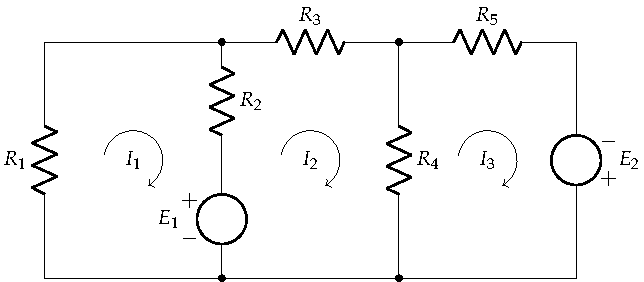
\includegraphics[height=3.7cm]{../figs/ej2_BT1.pdf}
  \end{center}

  \emph{Sol.:\; $I_1=\qty{-1.31}{\ampere};\, I_2=\qty{3.17}{\ampere};\, \qty{10.45}{\ampere}$}
		
\item Calcular el valor de $E$ que hace que $I_0=\qty{7.5}{\milli\ampere}$ en el
  circuito de la figura.

  Datos: $\; R_1 = \qty{8}{\ohm}$;\, $R_2 = \qty{7}{\ohm}$;\, $R_3 = \qty{4}{\ohm}$;\, $R_4 = \qty{6}{\ohm}$;\, $R_5 = \qty{6}{\ohm}$;\, $R_6 = \qty{12}{\ohm}$ 
  
  \begin{center}
    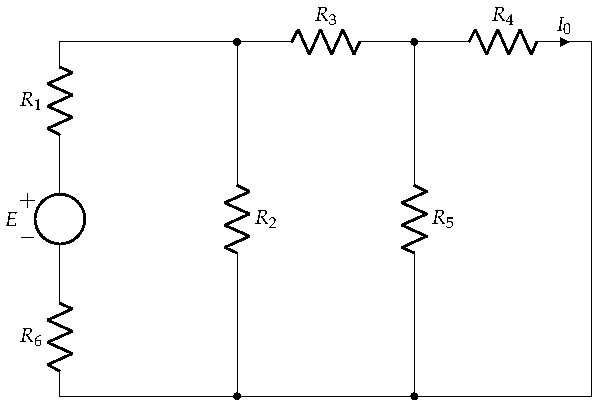
\includegraphics[height=5.5cm]{../figs/ej3_BT1.pdf}
  \end{center}
  
  \emph{Sol.:\; $U_s=\qty{0.705}{\volt}$}
		
\item Calcular la intensidad $I$ en el circuito de la figura.

    Datos: $\; R_1 = \qty{27}{\ohm}$;\, $R_2 = \qty{47}{\ohm}$;\, $R_3 = \qty{27}{\ohm}$;\, $E_1 = \qty{460}{\volt}$;\, $E_2 = \qty{200}{\volt}$
    
  \begin{center}
    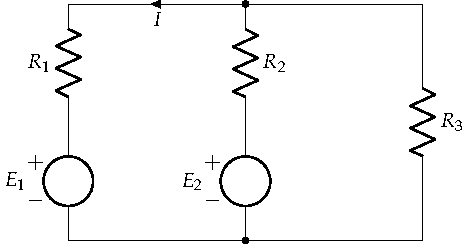
\includegraphics{../figs/ej4_BT1.pdf}
  \end{center}

  \emph{Sol.:\; $I=\qty{-8.77}{\ampere}$}
		
\item En el circuito de la figura obtener las intensidades de
  corriente señaladas primero mediante un análisis por el método de
  las mallas y posteriormente mediante un análisis por el método de
  los nudos.

  Datos: $\; R_1 = \qty{2}{\ohm}$; $R_2 = \qty{1}{\ohm}$; $R_3 = \qty{4}{\ohm}$; $R_4 = \qty{5}{\ohm}$; $R_5 = \qty{3}{\ohm}$; $E_1 = \qty{10}{\volt}$; $E_2 = \qty{6}{\volt}$
  
  \begin{center}
    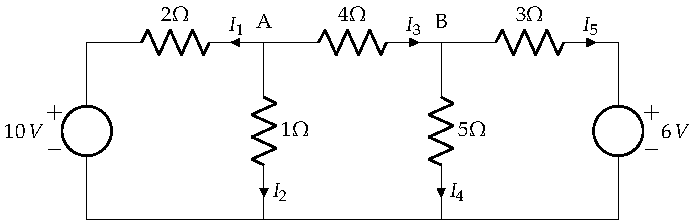
\includegraphics{../figs/ej8_BT1.pdf}
  \end{center}

  \emph{Sol.:\;
    $I_1=\qty{-3.31}{\ampere};\, I_2=\qty{3.37}{\ampere};\, I_3=\qty{-0.06}{\ampere};\, 
    I_4=\qty{0.73}{\ampere};\,  I_5=\qty{-0.79}{\ampere};\, $}
 	
\item Analizar el circuito de la figura mediante el método de las mallas, obteniendo la corriente de cada una de las ramas. Con este resultado, calcular la diferencia de potencial entre A y B, y realizar un balance de potencias comparando la potencia de los elementos activos y la de los elementos pasivos. 

Datos: $\; R_1 = R_2 = \qty{1}{\ohm};\, R_3 = \qty{2}{\ohm};\, R_4 = \qty{3}{\ohm};\, R_5=\qty{4}{\ohm};\, \epsilon_1=\qty{118}{\volt};\, \epsilon_2 = \qty{236}{\volt};\, \epsilon_3 = \qty{118}{\volt}$\\

  \begin{center}
    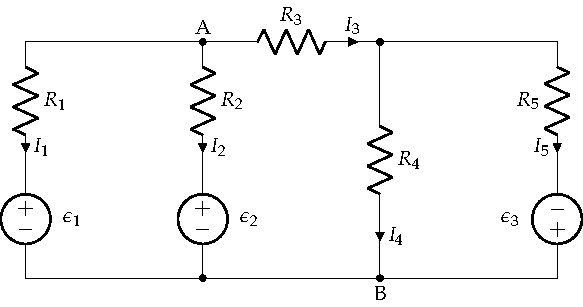
\includegraphics{../figs/mallas2.pdf}
  \end{center}

 \emph{Sol.:\;
    $I_1 = \qty{32}{\ampere};\, I_2 = \qty{-86}{\ampere};\, I_3 =\qty{54}{\ampere};\, I_4 = \qty{14}{\ampere};\, I_5 = \qty{40}{\ampere};\,
    U_{AB}=\qty{150}{\volt};\, P_g = P_R$}
 	
\item En el circuito de la figura, determinar:
  \begin{itemize}
  \item Todas las intensidades de rama señaladas
  \item Carga, polaridad y energía almacenada en los condensadores
  \item Balance de potencias
  \end{itemize}
    Datos: $\; R_i = \qty[parse-numbers=false]{i}{\ohm}$;\, $C_i = \qty[parse-numbers=false]{i}{\micro\farad}$;\, $E_1 = \qty{8}{\volt}$;\, $E_2 = \qty{6}{\volt}$;\, $E_3 = \qty{4}{\volt}$

  \begin{center}
    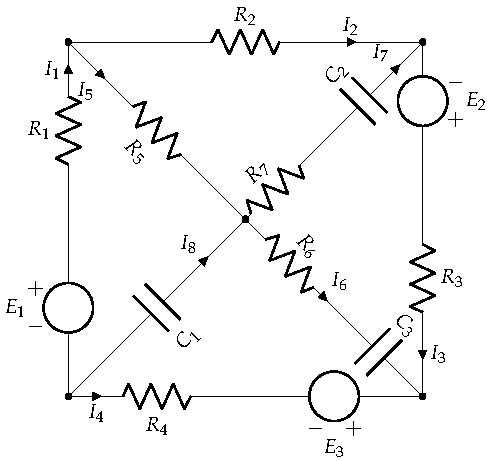
\includegraphics[height=7cm]{../figs/ej9_BT1.pdf}
  \end{center}

  \emph{Sol.:\;
    $I_1=I_2=I_3=-I_4=\qty{1}{\ampere};\,  I_5=I_6=I_7=\qty{0}{\ampere};\, Q_{1\si{\micro\farad}}=\qty{-7}{\micro\coulomb};\, Q_{2\si{\micro\farad}}=\qty{-4}{\micro\coulomb};\, Q_{3\si{\micro\farad}}=\qty{3}{\micro\coulomb};\, E_{1\si{\micro\farad}}=\qty{24.5}{\micro\joule};\, E_{2\si{\micro\farad}}=\qty{4}{\micro\joule};\, E_{3\si{\micro\farad}}=\qty{1.5}{\micro\joule}$}

\item Aplicar el método de los nudos en el circuito de la figura para
  determinar:
  \begin{itemize}
  \item Los potenciales de los nudos A, B, C y D.
  \item Las intensidades de corriente señaladas.
  \item Carga, polaridad y energía almacenada en los condensadores,
    supuestos sin carga inicial.
  \end{itemize}
  Datos:
  $\; R_i = \mathrm{i\ } \Omega;\, C_i = \mathrm{i\ } \si{\micro\farad};\, E_1 = \qty{6}{\volt};\, E_2
  = \qty{18}{\volt};\, E_3 = \qty{6}{\volt}$
  \begin{center}
    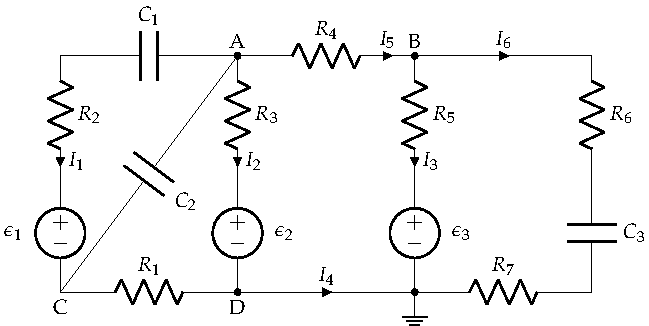
\includegraphics[]{../figs/nudos_condensadores.pdf}
  \end{center}

  \emph{Sol.:\;
    $U_A=\qty{15}{\volt};\, U_B=\qty{11}{\volt};\, U_C=U_D=\qty{0}{\volt};\, I_1=I_6=\qty{0}{\ampere};\, I_2=I_4=\qty{-1}{\ampere};\, I_3=I_5=\qty{1}{\ampere};\,
    q_1=\qty{9}{\micro\coulomb};\, q_2=\qty{30}{\micro\coulomb};\, q_3=\qty{33}{\micro\coulomb};\, E_{C1}=\qty{40.5}{\micro\joule};\,
    E_{C2}=\qty{225}{\micro\joule};\, E_{C2}=\qty{181.5}{\micro\joule}$}

\item En el circuito de la figura, donde se sabe
  que la carga inicial de los condensadores era de
  $\qty{10}{\micro\coulomb}$ para $C_1$ y de
  $\qty{20}{\micro\coulomb}$ para $C_2$ con las polaridades indicadas,
  se pide determinar:
  \begin{itemize}
  \item Intensidades de corriente señaladas
  \item Potenciales en los puntos A, B, C, D, E y F
  \end{itemize}

  Datos:
  $\;\epsilon_1=\SI{90}{\volt};\, \epsilon_2=\SI{60}{\volt};\,
  \epsilon_3=\SI{30}{\volt};\, R_{1}= R_2 = R_3 =
  \SI{10}{\ohm};\, R_{4}= R_5 = \SI{30}{\ohm};\, C_{1}=
  \SI{10}{\micro\farad};\, C_{2}= \SI{20}{\micro\farad};\, L_1 =
  \SI{1}{\micro\henry}$

  \begin{center}
    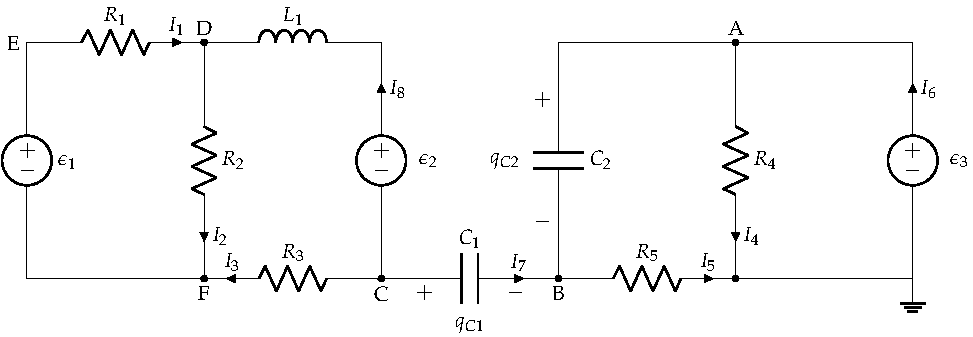
\includegraphics[scale = 0.9]{../figs/mallas_carga_inicial.pdf}
  \end{center}

\emph{Sol.:\;
  $I_1=\qty{4}{\ampere};\, I_2=\qty{5}{\ampere};\, I_3=\qty{-1}{\ampere};\, I_4=I_6=\qty{1}{\ampere};\, I_5=I_7=\qty{0}{\ampere};\, I_8=\qty{1}{\ampere};\, U_A=\qty{30}{\volt};\, U_B=\qty{0}{\volt};\,
  U_C=\qty{1}{\volt};\, U_D=\qty{61}{\volt};\, U_E=\qty{101}{\volt};\, U_F=\qty{11}{\volt};\,$}

\item En el circuito de la figura, los condensadores se conectaron sin
  carga. Mediante el método de las mallas, se debe determinar:
  \begin{itemize}
  \item Intensidades de corriente señaladas
  \item Potenciales en los puntos A, B, C y D
  \item Polaridades, cargas, y energías de los condensadores
  \item Balance de potencias
  \end{itemize}
  Datos:
  $\; \epsilon_{1}=\qty{118}{\volt};\, \epsilon_{2}=\qty{236}{\volt};\, \epsilon_{3}=\qty{118}{\volt};\,
  R_{1}= \qty{4}{\ohm};\, R_{2}=R_{3}=\qty{1}{\ohm};\, R_{4}= \qty{3}{\ohm};\,
  R_{5}=\qty{2}{\ohm};\, C_{1}=C_{2}=C_{3}=\qty{2}{\micro\farad};\, L_1 = L_2 = L_3 = \qty{1}{\milli\henry}$
  \begin{center}
    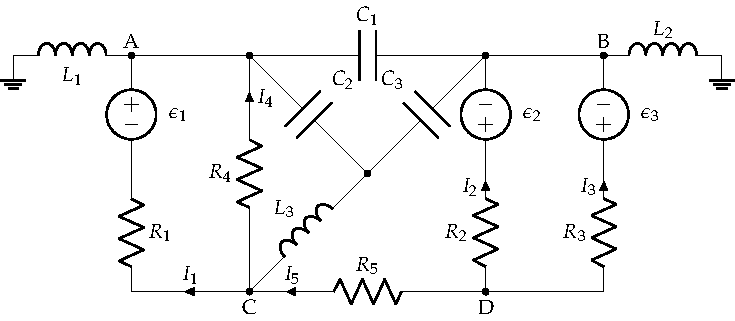
\includegraphics{../figs/mallas_condensadores.pdf}
  \end{center}

  \emph{Sol.:\;
    $I_1=\qty{40}{\ampere};\, I_2=\qty{-86}{\ampere};\, I_3=\qty{32}{\ampere};\, I_4=\qty{14}{\ampere};\, I_5=\qty{54}{\ampere};\, U_A=U_B=\qty{0}{\volt};\,
    U_C=\qty{42}{\volt};\, U_D=\qty{150}{\volt};\, U_{C1}=\qty{0}{\volt};\, q_1=\qty{0}{\coulomb};\, E_{C1}=\qty{0}{\joule};\, U_{C2}=\qty{-42}{\volt};\,
    q_2=\qty{84}{\micro\coulomb};\, E_{C2}=\qty{1.76}{\milli\joule};\, U_{C3}=\qty{-42}{\volt};\, q_3=\qty{84}{\micro\coulomb};\, E_{C3}=\qty{1.76}{\milli\joule};\, P_g = P_R$}

\item En el circuito de la figura, se debe determinar:
  \begin{itemize}
  \item Las ecuaciones para el cálculo de las intensidades
  \item Todas las intensidades indicadas
  \item Potenciales en todos los nudos
  \item Carga y energía almacenada en los condensadores
  \end{itemize}

  Datos: $\; R_1 = \qty{2}{\ohm}$;\, $R_2 = \qty{4}{\ohm}$;\, $R_3 = \qty{2}{\ohm}$;\, $R_4 = \qty{1}{\ohm}$;\, $R_5 = \qty{2}{\ohm}$;\, $R_6 = \qty{1}{\ohm}$;\, $E_1 = \qty{8}{\volt}$;\, $E_2 = \qty{8}{\volt}$;\, $C_i = \qty[parse-numbers=false]{i}{\micro\farad}$
  
  \begin{center}
    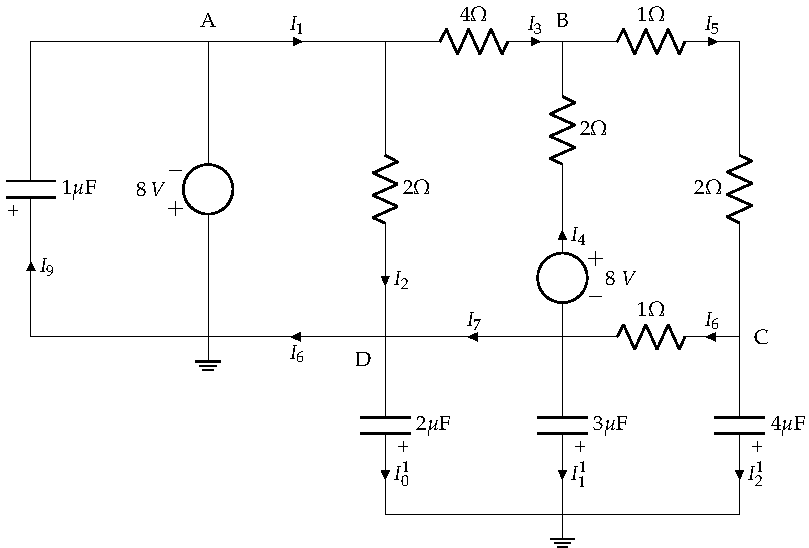
\includegraphics[height=8cm]{../figs/ej11_BT1.pdf}
  \end{center}

  \emph{Sol.:\;
    $I_1=I_8=\qty{-6.5}{\ampere};\, I_2=\qty{-4}{\ampere};\, I_3=I_7=\qty{-2.5}{\ampere};\, I_4=\qty{3}{\ampere};\, I_5=I_6=\qty{0.5}{\ampere};\, U_A=\qty{-8}{\volt};\,
    U_B=\qty{2}{\volt};\, U_C=\qty{0.5}{\volt};\, U_D=\qty{0}{\volt};\, Q_{1\si{\micro\farad}}=\qty{8}{\micro\coulomb};\, Q_{2\si{\micro\farad}}=Q_{3\si{\micro\farad}}=\qty{0}{\micro\coulomb};\, Q_{4\si{\micro\farad}}=\qty{-2}{\micro\coulomb};\, E_{1\si{\micro\farad}}=\qty{32}{\micro\joule};\, E_{2\si{\micro\farad}}=E_{3\si{\micro\farad}}=\qty{0}{\joule};\, E_{4\si{\micro\farad}}=\qty{0.5}{\micro\joule}$}

\newpage

\item En el circuito de la figura, se debe determinar:
  \begin{itemize}
  \item Las corrientes señaladas.
  \item El balance de potencias, diferenciando entre elementos activos
    y elementos pasivos.
  \item Los potenciales en los puntos A, B y C.
  \item La carga y polaridad en los condensadores, supuestos sin carga
    inicial.
  \end{itemize}
  Datos:
  $\; \epsilon_1 =\qty{1}{\volt};\, \epsilon_2 =\qty{7}{\volt};\, R_i = \qty{1}{\ohm};\, C_i = i\, \si{\micro \farad}$

  \begin{center}
    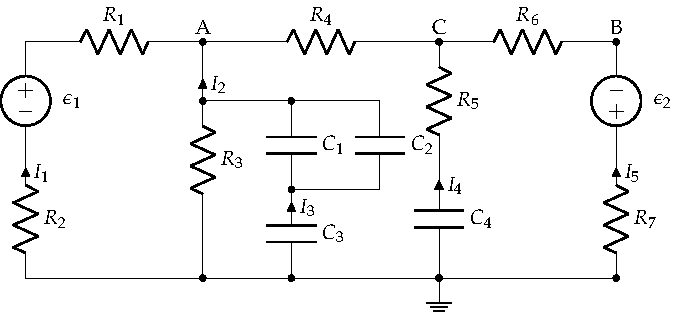
\includegraphics[height=5cm]{../figs/mallas_agrupacion_condensadores.pdf}
  \end{center}

  \emph{Sol.:\;
    $I_1=I_2=\qty{1}{\ampere};\, I_3=I_4=\qty{0}{\ampere};\, I_5=\qty{-2}{\ampere};\, \sum_\epsilon P_\epsilon = \sum_R P_R;\, U_A=\qty{-1}{\volt};\, U_B=\qty{-5}{\volt};\, U_C=\qty{-3}{\volt};\, q_1=\qty{0.5}{\micro\coulomb};\, q_2 = \qty{1}{\micro\coulomb};\, q_3=\qty{1.5}{\micro\coulomb};\, q_4=\qty{12}{\micro\coulomb}$}

\item El circuito de la figura está funcionando en régimen
  estacionario. Los condensadores estaban inicialmente
  descargados. Resuelve el circuito mediante el método que consideres
  conveniente para obtener los siguientes resultados:
  \begin{itemize}
  \item Las intensidades señaladas.
  \item Polaridad y energía almacenada en los condensadores.
  \item Balance de potencias.
  \end{itemize}
  Datos:
  $\; \epsilon_{1}=\qty{40}{\volt};\, \epsilon_{2}=\qty{22}{\volt};\, \epsilon_{3}=\qty{20}{\volt};\,
  C_{1}=C_{2}=C_{3}=\qty{2}{\micro\farad};\, R_{g1}=R_{g2}=R_{g3}=\qty{4}{\ohm};\,
  R_{1}=R_{2}=R_{3}=R_{4}=\qty{2}{\ohm};\, R_{5}=R_{6}=R_{7}=\qty{1}{\ohm}$
  \begin{center}
    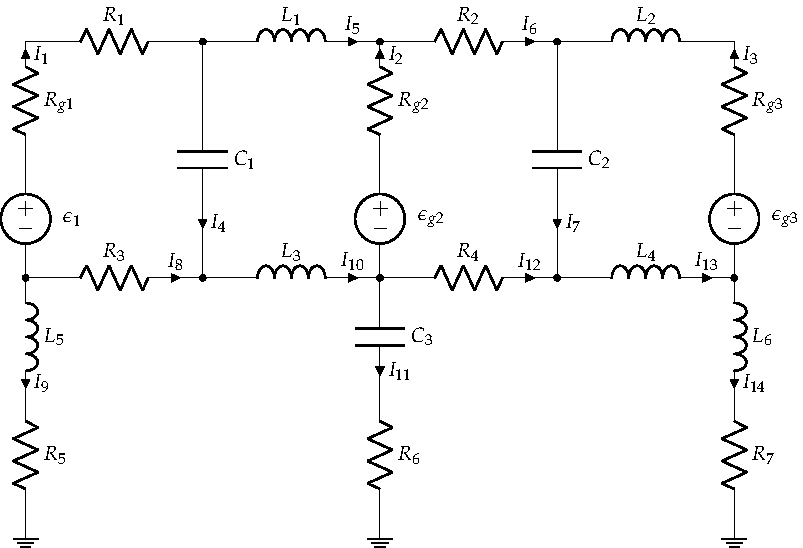
\includegraphics[height=8cm]{../figs/mallas_condensadores_bobinas.pdf}
  \end{center}
  \emph{Sol.:\;
    $I_1=I_5=\qty{2}{\ampere};\, I_2=I_3=I_8=I_{10}=\qty{-1}{\ampere};\,
    I_4=I_7=I_{11}=I_{12}=I_{13}=\qty{0}{\ampere};\, I_6=I_{14}=\qty{1}{\ampere};\, E_{C1}=\qty{0.676}{\milli\joule};\,
    E_{C2}=\qty{0.576}{\milli\joule}; \, E_{C3}=\qty{1}{\micro\joule}; P_g = P_R$}
 
\item En el circuito de la figura, obtener las
  intensidades de corriente señaladas mediante un análisis por el
  método de las mallas y mediante un análisis por el método de los
  nudos.

  Datos: $\; R_1 = \qty{9}{\ohm}$; $R_2 = \qty{4}{\ohm}$; $R_3 = \qty{18}{\ohm}$; $R_4 = R_5 = R_6 = \qty{20}{\ohm}$; $E_1 = \qty{16}{\volt}$; $I_g = \qty{2}{\ampere}$
  
  \begin{center}
    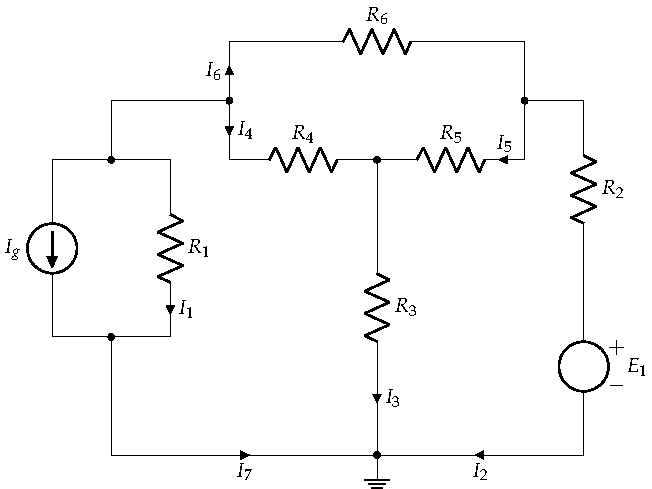
\includegraphics{../figs/ej12_BT1.pdf}
  \end{center}

  \emph{Sol.:\;
    $I_1=\qty{-0.74}{\ampere};\,I_2=\qty{-1.33}{\ampere};\,I_3=\qty{0.07}{\ampere};\,I_4=\qty{-0.39}{\ampere};\,I_5=\qty{0.46}{\ampere};\,I_6=\qty{-0.87}{\ampere};\,I_7=\qty{1.26}{\ampere}$}

\item Calcular la intensidad que circula por la resistencia de 30$\,\Omega$ del circuito de la figura aplicando el principio de
  superposición.

  Datos: $\; R_1 = \qty{20}{\ohm}$; $R_2 = \qty{30}{\ohm}$; $R_3 = \qty{20}{\ohm}$; $E_1 = \qty{32}{\volt}$; $E_2 = \qty{64}{\volt}$; $I_g = \qty{4}{\ampere}$
  
  \begin{center}
    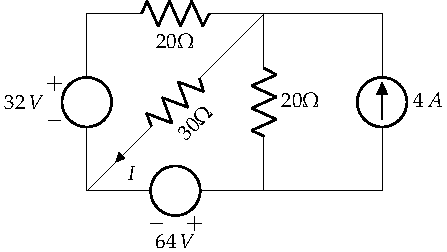
\includegraphics{../figs/ej16_BT1.pdf}
  \end{center}
  
  \emph{Sol.:\; $I=\qty{2.2}{\ampere}$}

\item Obtener el generador equivalente de Thévenin del circuito de la
  figura respecto de A y B. A partir de este generador, calcula la
  resistencia a colocar en A-B para obtener la máxima potencia,
  calculando esta potencia y la potencia entregada por el generador
  $\epsilon$.

  Datos:
  $\; \epsilon = \qty{54}{\volt};\; R_1 = R_4 = \qty{8}{\ohm};\;
  R_2 = R_3 = \qty{10}{\ohm}$

  \begin{center}
    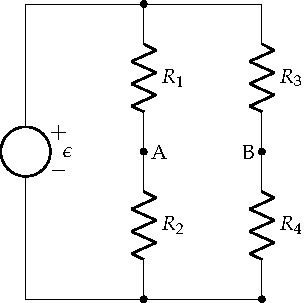
\includegraphics{../figs/Thevenin2}
  \end{center}

    \emph{Sol.:\;
      $R_{AB} = \dfrac{80}{9}\,\si{\ohm}; \; P_R = \qty{1.0125}{\watt}; \;
      P_\epsilon = \qty{2.025}{\watt}$}

  \item Determinar el equivalente Thévenin del circuito de la figura
    entre los nudos A-B. ¿Qué resistencia habría que conectar en
    dichos terminales para transferir la máxima potencia? ¿Cuál sería
    dicha potencia?

    Datos: $\; R_1 = R_2 = \qty{4}{\ohm}$; $R_3 = \qty{2}{\ohm}$; $E = \qty{10}{\volt}$; $I_g = \qty{8}{\ampere}$
    
    \begin{center}
      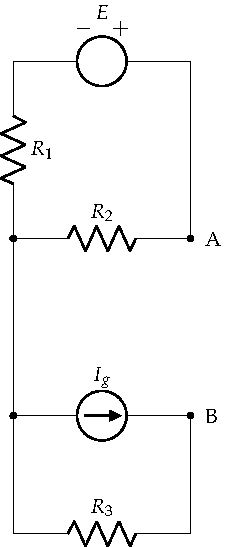
\includegraphics{../figs/ej17_BT1.pdf}
    \end{center}

    \emph{Sol.:\;
      $\epsilon_{th}=5-16=\qty{-11}{\volt};\; R_{th}=\qty{4}{\ohm};\;
      R_L=\qty{4}{\ohm};\;P_{max}=\qty{7.56}{\watt}$}


  \item Obtener el generador equivalente de Thévenin del circuito de la figura respecto de A y B.
  
    Datos: $\; I_g=\qty{10}{\ampere};\; R_1=\qty{1}{\ohm};\; \alpha=5$
    \begin{center}
      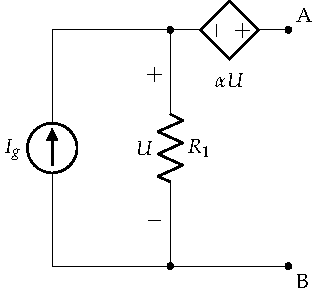
\includegraphics[height=4.5cm]{../figs/Thevenin1.pdf}
    \end{center}

    \emph{Sol.:\; $\epsilon_{th}=\qty{60}{\volt};\;R_{th}=\qty{62}{\ohm}$}

  \item En el circuito de la figura, calcular:
    \begin{itemize}
    \item La corriente del generador equivalente de Norton respecto de
      A y B, $I_N$.
    \item La resistencia del generador equivalente de Norton respecto
      de A y B, $R_N$.
    \item La resistencia de carga que se debe conectar entre A y B
      para conseguir la máxima potencia disponible, y el valor de esta
      potencia.
    \end{itemize}
    Datos:
    $\; R = \qty{1}{\ohm};\; \epsilon_g = \qty{10}{\volt};\; \alpha = \qty{2}{\ohm};\; \beta = 1$

    \begin{center}
      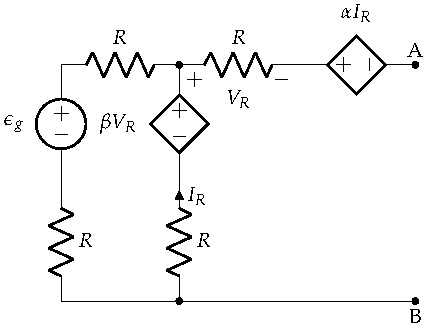
\includegraphics[height=4.5cm]{../figs/norton.pdf}
    \end{center}


\emph{Sol.:\;
  $I_N=\dfrac{10}{3}\,\si{\ampere};\; R_N=\qty{3}{\ohm};\; R_L=\qty{3}{\ohm};\;
  P_L=\qty{5.56}{\watt}$}

\end{enumerate}

%%% Local Variables:
%%% mode: latex
%%% TeX-master: "enunciados_ejercicios_TC"
%%% ispell-local-dictionary: "castellano"
%%% End:


% \chapter{Corriente alterna monofásica}

% \section*{Ejercicios}
	
\begin{enumerate}
		
\item En un circuito serie $RL$ con $R=5\Omega$ y $L=0.06H$, la
  tensión en bornes de la bobina es $u_L(t)=15\sin(200\,t)$
  V. Determinar:
  \begin{itemize}
  \item La tensión total
  \item Intensidad de corriente
  \item Ángulo de desfase de la intensidad respecto de la tensión
  \item Impedancia del circuito
  \end{itemize}
  \emph{Sol.:
    $\overline{Z_{eq}}=5+\mathrm{j}\,12\Omega;\;\overline{I}=0.88\phase{-90^\circ}A;\;\overline{U}=11.48\phase{-22.5304^\circ}
    V;\; \phi=67.4696^\circ$}

\item Una resistencia de \qty{5}{\ohm} y un condensador se unen en
  serie. La tensión en la resistencia es :
  $u_R(t) = 25 \cdot \sin(2000t + \pi/6)$. Si la corriente está
  adelantada \ang{60} respecto de la tensión aplicada, ¿cuál es el
  valor de la capacidad C del condensador?.  \emph{Sol.:
    $C = \SI[parse-numbers = false]{100\sqrt{3}/3}{\micro\farad}$}
  

\item Para determinar las constantes R y L de una bobina, se conecta
  en serie con una resistencia de \qty{25}{\ohm} y al conjunto se le
  aplica una fuente de tensión de \qty{120}{\volt} a \qty{60}{\hertz},
  se miden las tensiones en bornes de la resistencia y de la bobina,
  dando los valores $U_R = \qty{70.8}{\volt}$ y
  $U_B = \qty{86}{\volt}$. ¿ Cuáles son las constantes de la bobina en
  cuestión?.

  \emph{Sol.: $R = \qty{5}{\ohm}; L = \qty{79.5}{\milli\henry}$}

\item Un circuito serie RLC con $R = {5}{\Omega}$ , $L = {0.02}{H}$ y
  $C={80}{\mu F}$, tiene aplicada una tensión senoidal de frecuencia
  variable. Determinar los valores de la pulsación $\omega$ para los
  cuales la corriente:
  \begin{itemize}
  \item Adelanta {45}{$^\circ$} a la tensión
  \item Está en fase con ella
  \item Retrasa {45}{$^\circ$}
  \end{itemize}
  \emph{Sol.:
    $\omega=675.39\,rad/s;\; \omega=790.57\,rad/s;\,
    \omega=925.39\,rad/s$}

\item Determinar el triángulo de potencias de un circuito al que se le
  aplica una tensión $u(t)=340 \cdot \cos(\omega t - 60^\circ)$ V y
  circula una intensidad de corriente
  $i(t)= 13.3 \cdot \cos(\omega t-48.7^\circ)$.  \emph{Sol.  P =
    \qty{2217.17}{\watt}; Q = \qty{-443.03}{\voltampere_r}; S =
    \qty{2261}{\voltampere} }

\item En el esquema de la figura los elementos tienen los siguientes
  valores:
  \begin{align*}
    R_1 &= R_2 = R_3 = {10}{\Omega}\\
    X_1 &= X_2 = {1}{\Omega}\\
    R_L &= X_L = {1}{\Omega}
  \end{align*}
  Sabiendo que $U_{CD} = {200}{V}$ se debe calcular:
  \begin{itemize}
  \item Intensidades de corriente $I$, $I_1$, $I_2$ e $I_3$ {en forma
      fasorial}, tomando $U_{CD}$ como referencia de fase
  \item Lectura de los vatímetros $W_1$ y $W_2$
  \end{itemize}
  \begin{center}
    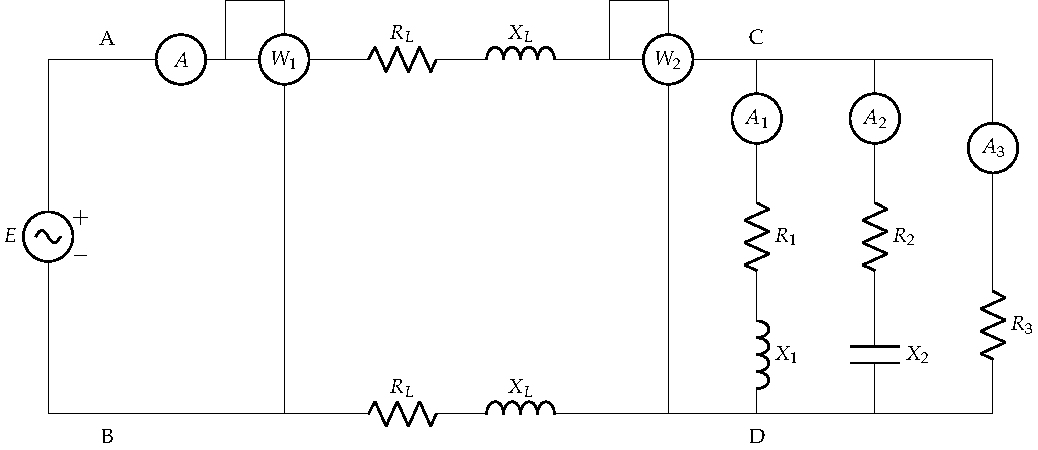
\includegraphics[width=\linewidth]{../figs/ej8_BT2.pdf}
  \end{center}

  \emph{Sol.:
    $\overline{I_1}=19.90\phase{-5.7106^\circ}\,A;\;
    \overline{I_2}=19.90\phase{5.7106^\circ}\,A;\;
    \overline{I_3}=20\phase{0^\circ}\,A;\;\overline{I}=59.60\phase{0^\circ}\,A;\;W_1=19024.32\,W;\;
    W_2=11920\,W$}

\item En el circuito de la figura, los amperímetros $A_1$ y $A_2$
  marcan ${4.5}{A}$ y ${6}{A}$, respectivamente; el voltímetro,
  ${150}{V}$ y el vatímetro ${900}{W}$. Sabiendo que la frecuencia del
  generador es de ${250}{Hz}$ y el f.d.p. de la impedancia $Z$ es de
  0.8 en retraso, se pide calcular:
  \begin{itemize}
  \item Valores de R, C y Z en forma compleja
  \item La tensión del generador
  \end{itemize}
  \begin{center}
    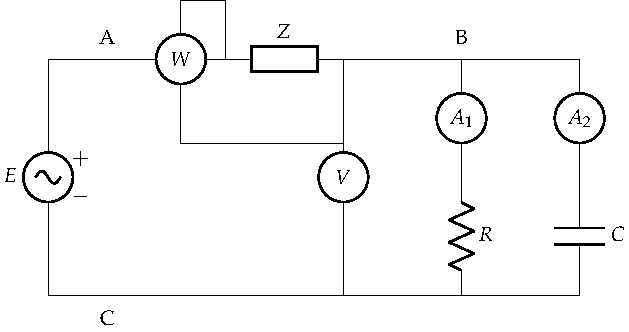
\includegraphics{../figs/ej9_BT2.pdf}
  \end{center}

  \emph{Sol.:
    $\overline{R}=33.33\phase{0^\circ}\Omega;
    \,\overline{X_c}-\mathrm{j}\,25\Omega;\,\overline{Z}=16+\mathrm{j}\,12\Omega;\,\overline{U_{AC}}=212.13\phase{45^\circ}
    V$}

\item En el circuito de la figura, determinar las lecturas de los aparatos de medida y el balance de potencias activas y reactivas, así como el triángulo global de potencias.\\
Datos: $e(t)=100\sqrt{2}\cos(\omega\,t)$; $R_1=2\Omega$;
$R_2=4\Omega$; $\omega\,L_1=3\Omega$; $\omega L_2=4\Omega$.

  \begin{center}
    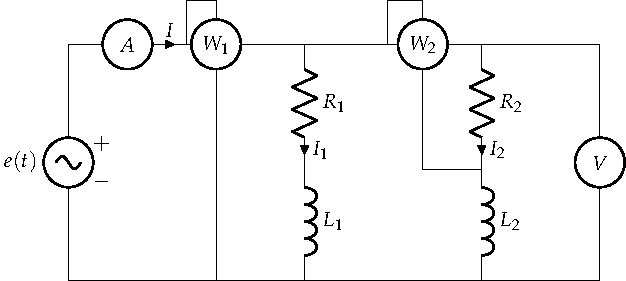
\includegraphics{../figs/ej11_BT2.pdf}
  \end{center}
    
  \emph{Sol.:
    $V=100\,V;\;A = 45.20
    A;\;W_1=2788.31W;\;W_2=1250.33\,W;\,P_{R1}=1539.02
    W;\;P_{R2}=1250.33 W;\,Q_{L1}=2308.52 VAr;\;Q_{L2}=1250.33
    VAr;\,P_T=2789.35 W;\,Q_T=3558.82
    VAr;\;\overline{S_T}=2789.35+\mathrm{j}3558.82 VA$}

\item El circuito de la figura tiene carácter inductivo.  La
  impedancia de la línea es $Z={10\sqrt{2}}{\Omega}$ con
  f.d.p. $\sqrt{2}/2$ en retraso. Tomando como referencia de fases la
  intensidad total $\overline{I}$, se pide calcular:
  \begin{itemize}
  \item Potencia activa y reactiva consumida por $Z$
  \item Expresiones complejas de las intensidades medidas por los
    amperímetros $A$, $A_1$, $A_2$ y $A_3$
  \item Expresiones complejas de las tensiones $\overline{U_{AB}}$,
    $\overline{U_{AC}}$ y $\overline{U_{CB}}$
  \item Valores de $R_1$, $X_1$, $R_2$, $R_3$ y $X_3$
  \end{itemize}
  Datos:
  $A = {5\sqrt{5}}{A};\; A_1 = {5\sqrt{2}}{A};\;A_2 = {5}{A};\;A_3 =
  {\sqrt{10}}{A};\;U_{AB} = {247}{V};\;W_1 = {2350}{W};\;R_1 = R_3$
  \begin{center}
    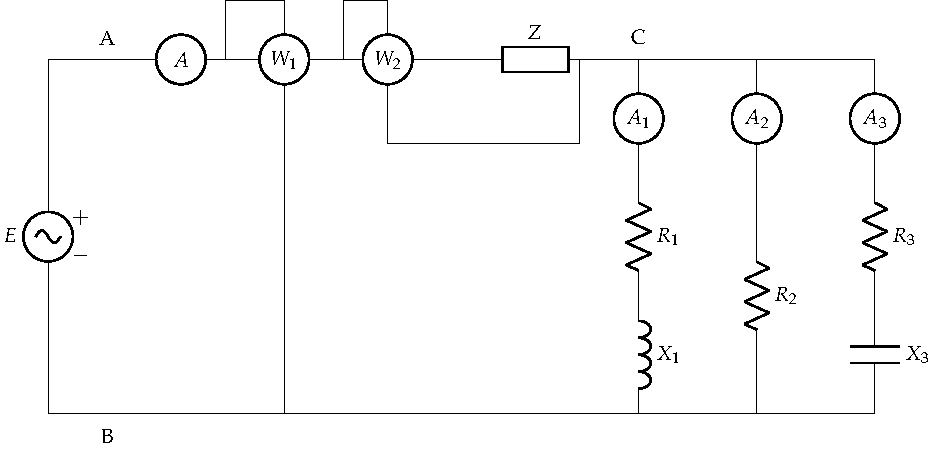
\includegraphics[width=0.8\linewidth]{../figs/ej17_BT2.pdf}
  \end{center}
  \emph{Sol.:
    $P_z=1250\,W;\;Q_z=1250\,VAr;\;\overline{I}=11.18\phase{0^\circ}A;\;
    \overline{I_1}=7.07\phase{-34.6711^\circ}A;\;
    \overline{I_2}=5\phase{10.3289^\circ}A;\;\overline{I_3}=3.16\phase{81.8940^\circ}A;\;
    \overline{U_{AB}}=247\phase{31.6823^\circ}V;\;
    \overline{U_{AC}}=158.11\phase{45^\circ}\,V;\;
    \overline{U_{CB}}=100\phase{10.3289^\circ}
    V;\;R_1=R_3=10\Omega;\;R_2=20\Omega;
    X_1=10\Omega;\;X_3=-30\Omega$}

\item La potencia reactiva del circuito de la figura es
  $\qty{80}{\voltampere_r}$ de tipo capacitivo. La tensión en la
  impedancia Z está en fase con la intensidad $I_1$ y las lecturas de
  los aparatos son $A = \qty{4}{\ampere}$, $V = \qty{50}{\volt}$,
  $W = \qty{200}{\watt}$. Sabiendo que $R_1 = \qty{10}{\ohm}$ y
  $X_2 = \qty{50}{\ohm}$, calcula:

  \begin{enumerate}
  \item Las corrientes $I_1$, $I_2$, $I_3$ en forma fasorial.
  \item Las reactancias $X_1$, $X_3$, y la impedancia $\overline{Z}$.
  \item La fuerza electromotriz $\overline{\epsilon}$.
  \end{enumerate}
  \begin{center}
    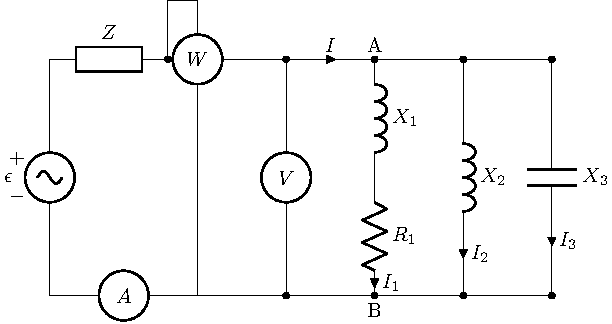
\includegraphics{../figs/BT2_circuitoCapacitivo}
  \end{center}
  \emph{Sol.
    $\overline{I} =
    \qty[parse-numbers=false]{4\phase{\ang{0}}}{\ampere};
    \overline{I}_1 =
    \qty[parse-numbers=false]{2\sqrt{5}\phase{\ang{-26.56}}}{\ampere}
    ; \overline{I}_2 =
    \qty[parse-numbers=false]{1\phase{\ang{-90}}}{\ampere} ; X_1 =
    \qty{5}{\ohm}; X_3 =
    \qty[parse-numbers=false]{\frac{50}{3}}{\ohm}; \overline{Z} =
    \qty[parse-numbers=false]{10 - j5}{\ohm}; $ }

\item Un motor monofásico de $S = {10}{kVA}$ y $fdp = 0.8$ está
  alimentado por una fuente de ${230}{V}$ a $f = {50}{Hz}$.  Calcular:
  \begin{itemize}
  \item El valor eficaz de la corriente absorbida por el motor
  \item La potencia aparente del generador
  \item La capacidad del condensador necesario para compensar el
    factor de potencia a la unidad
  \item El valor eficaz de la corriente absorbida por el conjunto
    condensador-motor
  \item La potencia aparente del generador necesario una vez conectado
    el condensador del tercer apartado
  \item Compara de forma razonada los resultados de los apartados 4 y
    5 con los valores calculados en los apartados 1 y 2
  \end{itemize}
  \emph{Sol.:
    $I= {43.5}{A};\; S_g = {10}{kVA};\;C={361}{\mu F};\, I'=34.78A;\,
    S_g' = {8000}{kVA}$}

\item Un generador de corriente alterna monofásica ($f=50$ Hz)
  alimenta a dos cargas a través de una línea de cobre. Esta línea, de
  resistividad $\rho=21$ m$\Omega$ mm$^2$/m, tiene una longitud de 100
  m y una sección de 16 mm$^2$. Las dos cargas, cuya tensión de
  alimentación es de 230 V, son dos motores, uno con potencia de 7 kW
  y f.d.p. de $0.65$, y otro con una potencia de 5 kW y f.d.p. de
  $0.85$. Con esta información, se pide calcular:
  \begin{itemize}
  \item Triángulo de potencias de cada carga y del conjunto de ambas
  \item Valor eficaz de las corrientes en cada carga y de la corriente
    total
  \item Triángulo de potencias del generador
  \item Valor eficaz de la tensión en bornes del generador
  \item Capacidad del condensador a instalar en bornes de las cargas
    para mejorar el factor de potencia a $0.95$
  \item Valor eficaz de la corriente entregada por el generador una
    vez instalado el condensador
  \item Triángulo de potencias del generador una vez instalado el
    condensador
  \end{itemize}
  \emph{Sol.:
    $P_1=7000W;\;
    Q_1=8183.91VAr;\;S_1=10769.23VA;\;P_2=5000W;\;Q_2=5882.35VAr;\;S_2=3098.72VA;\;P_T=12000W;\;Q_T=11282.63VAr;\;S_T=16471.12VA;\,
    I_1=46.82\,A;\;I_2=25.58\,A;\;I_T=71.62\,A;\,P_g=13333.65
    W;\;Q_g=11282.63 VAr;\,S_g=17466.65 VA;\;U_g=243.88 V;\; C=441.66
    \mu F;\,I'=54.92 A;\;P_g'=12784.21 W;\;Q_g'=3944.21
    VAr;\;S_g'=13378.82 VA$}

\item Un generador de corriente alterna monofásica ($f = {50}{Hz}$)
  alimenta a dos cargas a través de una línea de cobre. Esta línea, de
  resistividad $\rho = {0.017}{\Omega mm^2/m}$, tiene una longitud de
  {40}{m} y una sección de {6}{mm$^2$}. Las dos cargas, cuya tensión
  de alimentación es de {200}{V}, son:
  \begin{enumerate}
  \item Un motor de {7}{kW} con f.d.p. {0,7}.
  \item Un grupo de lámparas fluorescentes con potencia total {200}{W}
    y f.d.p. {0,5}.
  \end{enumerate}
  Se pide:
  \begin{itemize}
  \item Esquema del circuito señalando adecuadamente los elementos,
    corrientes y tensiones
  \item Potencias activa, reactiva y aparente de cada carga
  \item Valor eficaz de las corrientes en cada carga, y de la
    corriente total
  \item Potencia activa y reactiva entregada por el generador
  \item Valor eficaz de la tensión en bornes del generador
  \item Capacidad necesaria a instalar en bornes de las cargas para
    mejorar el factor de potencia de las mismas a la unidad
  \item Valor eficaz de la tensión en bornes del generador, y potencia
    aparente entregada por el mismo una vez instalada la capacidad
    determinada en el apartado anterior
  \end{itemize}
  \emph{Sol.:
    $P_M = {7000}{W};\; Q_M = {7141.43}{VAr};\; S_M ={10000}{VA};\;
    P_F = {200}{W};\; Q_F = {346.41}{VAr};\; S_F ={400}{VA};\;I_M =
    {50}{A};\; I_F = {2}{A};\; I_T = {51.94}{A};\;P_g =
    {7811.50}{W};\; Q_g = {7487.8}{VAr};\; U_g = {208.33}{V};
    C={595.86}{\mu F};\; U_g' = {207.92}{V};\; S_g' = {7485.12}{VA}$ }

\item Un generador de corriente alterna ($f = \SI{50}{\hertz}$)
  alimenta una instalación eléctrica a través de una línea de cobre
  ($\rho = \SI{0.017}{\ohm\milli\meter\squared\per\meter}$) de
  $\SI{25}{\milli\meter\squared}$ de sección. La instalación eléctrica
  está compuesta por un motor de $S_m = \SI{10}{\kilo\voltampere}$ y
  $\mathrm{fdp} = 0.8$, una instalación de alumbrado fluorescente de
  $P_f = \SI{800}{\watt}$ y $\mathrm{fdp} = 0.9$, y diversas cargas
  electrónicas con una potencia conjunta $P_e = \SI{540}{\watt}$ y
  $\mathrm{fdp} = 0.5$ en retraso.

  Suponiendo que las cargas trabajan a su tensión nominal de
  $\SI{230}{\volt}$ y que están situadas a $\SI{100}{\meter}$ del
  generador, calcule:

  \begin{enumerate}
  \item Triángulo de potencias total de las cargas ($P_T$, $Q_T$,
    $S_T$) y factor de potencia.
  \item Valor eficaz de la corriente que circula por la línea.
  \item Potencia disipada en la línea.
  \item Triángulo de potencias del generador ($P_g$, $Q_g$, $S_g$) y
    factor de potencia.
  \item Valor eficaz de la tensión de salida del generador.
  \item Capacidad del banco de condensadores a instalar en bornes de
    la carga necesario para reducir la corriente que circula por la
    línea a un valor de $\SI{45}{\ampere}$.
  \end{enumerate}

  Independientemente del resultado obtenido, suponga que la capacidad
  instalada es $C = \SI{172}{\micro\farad}$. En estas condiciones,
  calcule:
  \begin{enumerate}[resume]
  \item Potencia aparente de las cargas (incluyendo al banco de
    condensadores)
  \item Valor eficaz de la corriente que circula por la línea y
    potencia disipada en la misma.
  \item Triángulo de potencias del generador y factor de potencia.
  \item Tensión de trabajo del generador.
  \end{enumerate}
  \emph{Sol.
    $ S_T = \SI{11868.4}{\voltampere}; I = \SI{51.6}{\ampere}; P_L =
    \SI{362.1}{\watt}; S_g = \SI{12155.4}{\voltampere}; U_g =
    \SI{235.6}{\volt}; C = \SI{172.3}{\micro\farad}; S'_T =
    \SI{10350.1}{\voltampere}; I' = \SI{45}{\ampere}; S'_g =
    \SI{10599.2}{\voltampere}; U'_g = \SI{235.5}{\volt} $}

\item Calcular la corriente $i(t)$ del circuito de la figura.
  \begin{center}
    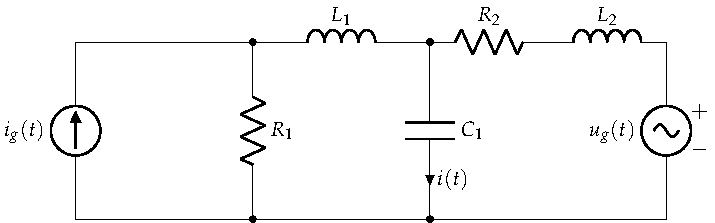
\includegraphics[width=\linewidth]{../figs/BT2_13.pdf}
  \end{center}

  \emph{Sol.: $i(t)=\sqrt{2}\,10\,\cos(100\,t) A$}

\item Del circuito de la figura obtener:
  \begin{itemize}
  \item Expresiones analíticas de las intensidades $i_1(t)$ e $i_2(t)$
  \item Potencia disipada por todas las resistencias
  \end{itemize}

  Datos: $e_g(t)=50\sqrt{2}\sin(1000\,t)$ V; $i_g(t)=10$ A;
  $R_1=R_2=2\Omega$; $R_3=7\Omega$; $L_1=L_2=1$ mH; $L_3=2$ mH
  \begin{center}
    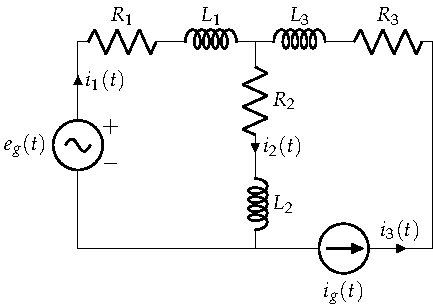
\includegraphics{../figs/ej18_BT2.pdf}
  \end{center}
  \emph{Sol.:
    $i_1(t)= -5+5\sqrt{10}\sin(1000t-0.46) A;\; i_2(t)=
    5+5\sqrt{10}\sin(1000t-0.46) A;\; i_3(t)= 10 A;\; P_T=1300\,W$}

\item En el circuito de la figura determina:
  \begin{itemize}
  \item $u_R(t)$ y $u_L(t)$
  \item Balance de potencias
  \end{itemize}
  Datos:
  $e_a(t) = {3\sqrt{2} \sin(10^3 t)} V;\,e_b(t) = {30\sqrt{2}
    \sin(10^4 t)} V;\,R = {30}{\Omega};\,L = {3}{mH}$
  \begin{center}
    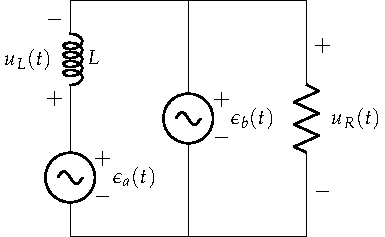
\includegraphics{../figs/superposicion2_ej.pdf}
  \end{center}

  \emph{Sol.:
    $u_R(t) = 30\sqrt{2}\sin(10^4 t) V;\; u_L(t) = 3\sqrt{2}\sin(10^3
    t) - 30\sqrt{2}\sin(10^4 t) V;\; P_R = {30}{W};\; P_\epsilon =
    {30}{W}$}

\item El circuito de la figura se encuentra en régimen
  permanente. Determinar analíticamente la expresión de $i(t)$, así
  como las potencias entregadas por los generadores y disipadas por
  las resistencias $R_1$ y $R_2$.

  Datos:
  $e_1(t) = {50 \sin(1000 t)} V;\; e_2(t) = {30}{V};\; R_1 =
  {6}{\Omega};\; R_2 = {6}{\Omega};\; L = {8}{mH};\; C = {10}{\mu F}$

  \begin{center}
    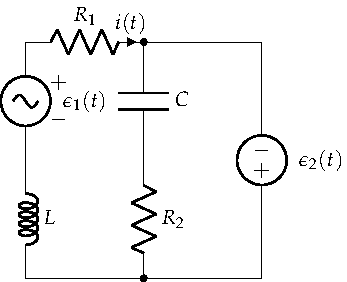
\includegraphics{../figs/superposicion1_ej.pdf}
  \end{center}
  \emph{Sol.:
    $i(t) = 5 + 5\sin(1000t - 0.9273){A};\; P_{R1} = {225}{W}; P_{R2}
    = {0}{W}; P_{\epsilon} = {225}{W}$}

\item   Obtén el generador equivalente de Thévenin del circuito de la figura
  respecto de A y B.

\begin{center}
  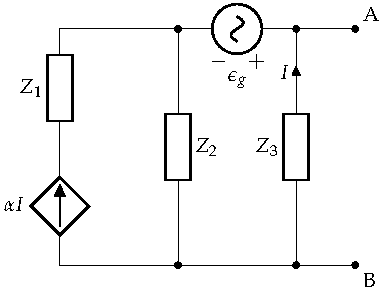
\includegraphics{../figs/Thevenin4}
\end{center}

Datos:
\begin{equation*}
  \overline{\epsilon_g} = \qty[parse-numbers=false]{12 - 16j}{\volt};
  \overline{Z}_1 = \qty[parse-numbers=false]{1 - j}{\ohm};
  \overline{Z}_2 = \qty[parse-numbers=false]{1 + j}{\ohm};
  \overline{Z}_3 = \qty[parse-numbers=false]{5 + 3j}{\ohm}
  \alpha = 2
\end{equation*}
\emph{Sol.
  $ \overline{\epsilon}_{th} = 11.66\phase{\ang{-59.04}}\si{\volt};
  \overline{Z}_{th} = 0.64 + 0.52j\si{\ohm}$}

\item Obtén el generador equivalente de Thévenin del circuito de la figura respecto de A y B. A partir de este generador, calcula la impedancia a colocar en AB para obtener la máxima potencia, calculando esta potencia.

\begin{minipage}{0.5\textwidth}
\begin{center}
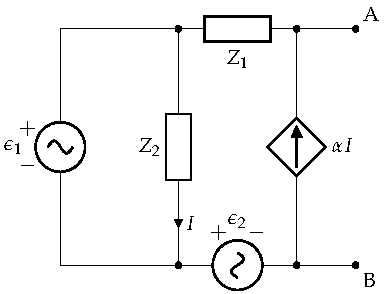
\includegraphics{../figs/Thevenin5}
\end{center}
\end{minipage}
\begin{minipage}{0.5\textwidth}
  \begin{align*}
    \overline{\epsilon_1} &= \SI[parse-numbers=false]{10\phase{0}}{\volt}\\
    \overline{\epsilon_2} &= \SI[parse-numbers=false]{10j}{\volt}\\
    \overline{Z}_1 &= \SI[parse-numbers=false]{4 - 3j}{\ohm}\\
    \overline{Z}_2 &= \SI[parse-numbers=false]{3 + 4j}{\ohm}\\
    \alpha &= 2
  \end{align*}
\end{minipage}

\emph{Sol. $
  \overline{\epsilon}_{th} = 11.66\phase{\ang{-59.04}}\si{\volt};
  \overline{Z}_{th} = 0.64 + 0.52j\si{\ohm}
  $}

\end{enumerate}
%%% Local Variables:
%%% mode: latex
%%% TeX-master: "enunciados_ejercicios_TC"
%%% ispell-local-dictionary: "castellano"
%%% End:


% \chapter{Sistemas trifásicos}

% \section*{Ejercicios}
\begin{enumerate}

\item El receptor trifásico de la figura tiene secuencia de fases
  inversa y tensión de línea 200$\sqrt{3}$ V. Su potencia activa es 12
  kW y el vatímetro 2 ($W_2$) indica 6 kW. Hallar:
  \begin{itemize}
  \item Valor de la impedancia $\overline{Z}$, en forma compleja.
  \item Fasores correspondientes a las intensidades de línea.
  \end{itemize}

\begin{center}
  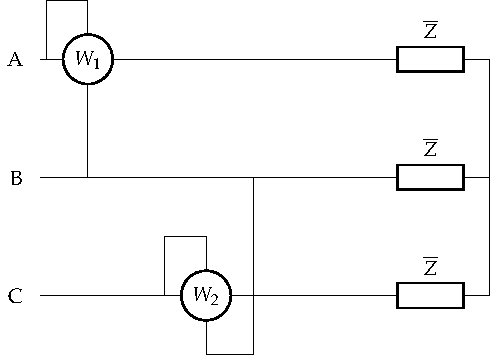
\includegraphics[width=0.45\linewidth]{../figs/ej6_BT3.pdf}
\end{center}

\emph{Sol.:
  $\overline{Z}=10\phase{0^\circ}\Omega;\;
  \overline{I_a}={20\phase{-90^\circ}\;\text{A}};
  \overline{I_b}={20\phase{30^\circ}\;\text{A}};
  \overline{I_c}={20\phase{150^\circ}\;\text{A}}$}


\item En el sistema trifásico de la figura de secuencia de fases
  directa y $f=60$ Hz, el receptor equilibrado disipa una potencia
  total $P_T =51984$ W con un factor de potencia de 0,6 en
  retraso. Sabiendo que el amperímetro indica 76$\sqrt{3}$ A,
  determinar:
  \begin{itemize}
  \item Lecturas de los vatímetros 1 y 2
  \item Valor de la impedancia $\overline{Z}$ en forma compleja
  \item Capacidad mínima para mejorar el factor de potencia a 0,95
  \end{itemize}
  \begin{center}
    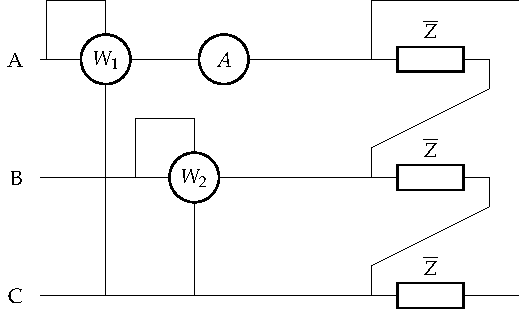
\includegraphics[width=0.5\linewidth]{../figs/ej4_BT3.pdf}
  \end{center}
  \emph{Sol.:
    $ W_1=46000.65\,W;\; W_2=5983.35\,W;\;
    \overline{Z}=3+\mathrm{j}\,4\;\Omega;\; C_D=\qty{319.8}{\micro\farad}$}

\item En el sistema trifásico de la figura, de secuencia de fases
  inversa y tensión de línea 200$\sqrt{3}$ V, los dos receptores son
  equilibrados, con impedancias
  $\overline{Z_1} = 6+\mathrm{j}8\;\Omega$ y
  $\overline{Z_2} = 8+\mathrm{j}6\;\Omega$. Determinar:
  \begin{itemize}
  \item Lecturas de los amperímetros.
  \item Lecturas de los vatímetros y la potencia compleja total.
  \end{itemize}
  \begin{center}
    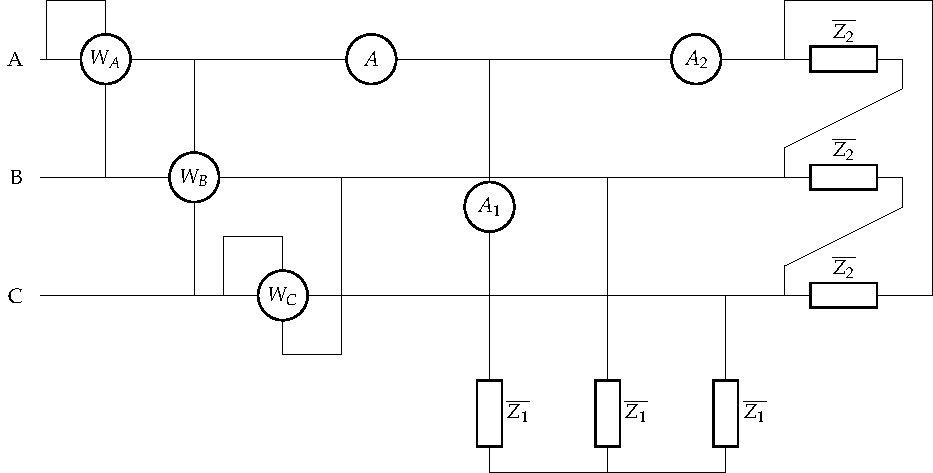
\includegraphics[width=.8\linewidth]{../figs/ej5_BT3.pdf}
  \end{center}

  \emph{Sol.:
    $A=79.40\,A;\;A_1=20\,A;\;A_2=60\,A;\; W_A={27007.43\;\text{W}};\;
    W_B={18013.85\;\text{W}};\;W_C={8993.58\;\text{W}};\;
    \overline{S_T}=36000+\mathrm{j}31200\,VA $}

\item El sistema trifásico de la figura es de 380 V a 50 Hz y
  secuencia de fases inversa. $\overline{Z}$ es un elemento pasivo
  ideal, tal que el factor global de potencia es la unidad. El motor
  es de 1,8 CV, rendimiento 90\% y factor de potencia 0,8. Determinar:
  \begin{itemize}
  \item Impedancia $\overline{Z}$ en forma compleja.
  \item Intensidad en el motor.
  \item Fasores intensidad de línea.
  \item Lectura de los aparatos de medida: V, A, W$_1$, W$_2$ y W$_3$.
  \end{itemize}
  \begin{center}
    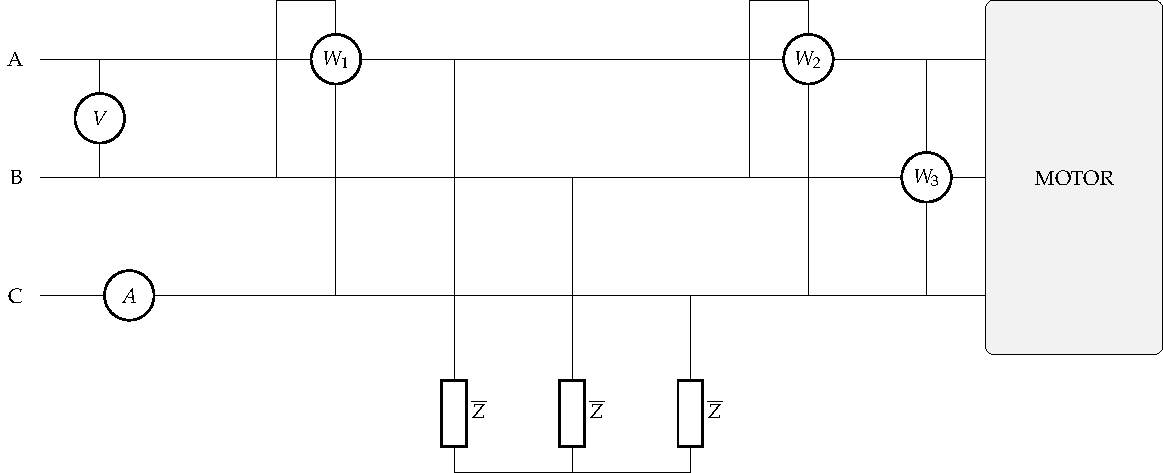
\includegraphics[width=\linewidth]{../figs/ej7_BT3.pdf}
  \end{center}

  \emph{Sol.:
    $\overline{Z}={-\mathrm{j}\,129.76}\;\Omega\text{/fase};\;
    I_M=2.83\,A;\;\overline{I_{a}}={2.27\phase{-90^\circ}\;\text{A}};\;
    \overline{I_{b}}={2.27\phase{30^\circ}\;\text{A}};\;
    \overline{I_{c}}={2.27\phase{150^\circ}\;\text{A}};\; W_1=0;\;
    W_2=-645.24W;\; W_3=645.24W$}

\item Una plantación agrícola emplea dos bombas sumergibles para
  extraer agua de un pozo y transportarla a través de un sistema de
  riego por goteo. Estas dos bombas están alimentadas a
  \SI{400}{\volt} por una línea trifásica en secuencia de fases
  directa y frecuencia $\SI{50}{\hertz}$. Una de las bombas funciona
  con un motor trifásico de $\SI{30}{\kilo\watt}$ y factor de potencia
  de 0.78. La otra bomba trabaja con un motor de
  $\SI{7.5}{\kilo\watt}$ y factor de potencia de 0.67.  La línea que
  alimenta estas dos bombas es resistiva, con resistividad
  $\rho = \SI{0.017}{\ohm\milli\meter\squared\per\meter}$, longitud de
  \SI{300}{m} y una sección de \SI{35}{\milli\meter\squared}.
 
  \begin{enumerate}
  \item Calcula el triángulo de potencias (potencia activa, reactiva,
    y aparente) de cada carga, y total de las cargas (a la salida de
    la línea).
  \item Calcula el \textbf{valor eficaz} de la corriente de línea de
    cada carga, y total.
  \item Determine la lectura de los siguientes aparatos de medida
    conectados a la entrada de las cargas:
    \begin{itemize}
    \item Un vatímetro en la fase A, midiendo tensión entre las fases
      A y C.
    \item Un vatímetro en la fase B, midiendo tensión entre las fases
      B y C.
    \item Un vatímetro en la fase C, midiendo tensión entre las fases
      B y A.
    \end{itemize}
  \item Calcule el triángulo de potencias a la entrada de la línea.
  \item Calcule el \textbf{valor eficaz} de la tensión a la entrada de
    la línea.
  \item Calcule los condensadores que se deben conectar a la salida de
    la línea para mejorar el factor de potencia del sistema hasta la
    unidad. Indique el modo de conexión.
  \end{enumerate}

  Una vez conectados los condensadores del último apartado:
  \begin{enumerate}[resume]
  \item Calcule el \textbf{valor eficaz} de la corriente de línea
    total.
  \item Calcule el triángulo de potencias a la entrada de la línea.
  \item Calcule el \textbf{valor eficaz} de la tensión a la entrada de
    la línea.
  \item Determine la lectura de los vatímetros descritos
    anteriormente.
  \end{enumerate}
  \emph{Sol.:
    $P_1 = {30}{kW};\; Q_1 = {24.07}{kVAr};\; S_1={38.46}{kVA};\; P_2
    = {7.5}{kW};\; Q_2 = {8.31}{kVAr};\; S_2 ={11.19}{kVA}; P_T=
    {37.5}{kW}; \;Q_T= {32.38}{kVAr};\; S_T = {49.55}{kVA};\; I_1 =
    {55.51}{A};\; I_2 = {16.15}{A};\; I_T= {71.52}{A};\; W_{A,AC} =
    {28.10}{kW}; \; W_{B,BC} = {9.40}{kW};\;W_{C, BA} =-
    {18.69}{kW};\; P_g = {39.74}{kW};\; Q_g= {32.38}{kVAr};\; S_g =
    {51.26}{kVA};\;U_g = {413.81}{V};\; C = {214.7}{\mu F/fase};\;
    I_T' = {54.13}{A};\; P_g' = {38.78}{kW};\; Q_g' = {0}{VAr};\; S_g'
    ={38.78}{kVA};\; U' = {413.66}{V};\; W_{A,AC}' = {18.75}{kW};\;
    W_{B,BC}' = {18.75}{kW};\; W'_{C,BA} = {0}{W}$ }
 
\item El circuito de la figura es de secuencia de fases directa y 50
  Hz. Determinar:
  \begin{enumerate}
  \item Potencias activas y reactivas totales.
  \item Capacidad mínima de los condensadores a instalar para mejorar
    el factor de potencia total hasta la unidad.
  \item Intensidades de línea, en forma fasorial, una vez mejorado el
    factor de potencia.
  \end{enumerate}
  \begin{minipage}{0.4\linewidth}
    Datos:

    \begin{align*}
      \overline{Z}_1 &= {100\phase{\ang{60}}}\unit{\ohm}\\
      W_1 &= \SI{300}{\watt}\\
      W_2 &= \SI{300}{\watt}\\
      V &= {\sqrt{3} \cdot 200}\unit{\volt}
    \end{align*}
  \end{minipage}
  \begin{minipage}{0.6\linewidth}
    \begin{center}
      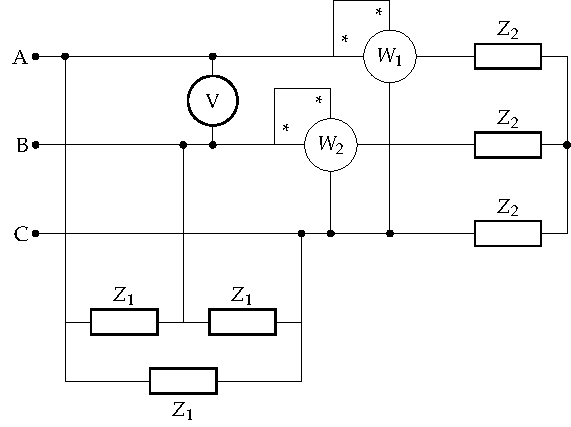
\includegraphics{../figs/ZyZt}
    \end{center}
  \end{minipage}
  
  \emph{Sol.:
  $P_T = {2400} W;\; Q_T =1800\sqrt{3}{VAr};\; C=27.57\,\mu
  F;\;\overline{I}_A = {4\phase{{90^\circ}}}{A}; \;
  \overline{I}_B={4\phase{{-30^\circ}}}{A};\; \overline{I}_C
  ={4\phase{{-150^\circ}}}{A}$}

  
\item En la figura dos vatímetros miden una carga trifásica inductiva
  equilibrada alimentada a una tensión $U = \SI{400}{\volt}$. El
  vatímetro $W_B$ indica una lectura de \SI{11320}{\watt}, y el
  vatímetro $W_C$ indica una lectura de \SI{1815}{\watt}. A partir de
  esta información se pide:

  \begin{enumerate}
  \item Determinar la secuencia de fases del sistema.
  \item Triángulo de potencias de la carga.
  \item Impedancia equivalente de la carga en estrella y en triángulo.
  \item Tensión de alimentación a la entrada de la línea $U_1$
    sabiendo que la línea de alimentación es resistiva pura con valor
    $R = \SI{0.1}{\ohm}$.
  \item Capacidad de los condensadores que se deben conectar en bornes
    de la carga para conseguir mejorar su factor de potencia a la
    unidad. Determinar las nuevas lecturas de los vatímetros $W_B$ y
    $W_c$.
  \end{enumerate}

\begin{center}
  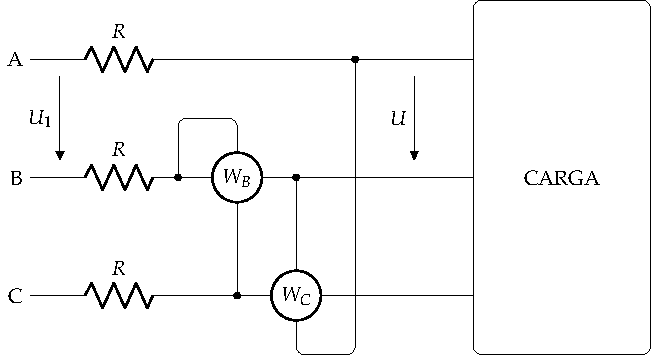
\includegraphics[width=0.6\linewidth]{../figs//BT3_10.pdf}
\end{center}

\textbf{Sol.: SFI; $ P = \qty{20825}{\watt}$;
  $Q = \qty{3143.7}{VA}_r$;
  $\overline{S} = 21060.9\phase{\ang{8.58}}\unit{VA}$;
  $\overline{Z}_{\triangle} = {22.8\phase{\ang{8.58}}}\unit{\ohm}$;
  $U_1 = \SI{405.21}{\volt}$; $C = \SI{20.85}{\micro\farad}$; }

\item Del circuito de la figura se sabe que tiene una secuencia de
  fases directa ABC. El amperímetro indica $\SI{5}{\ampere}$, el
  voltímetro $\SI{400}{\volt}$, y los vatímetros A y C muestran una
  lectura idéntica. Se pide:

  \begin{enumerate}
  \item Valor de la impedancia Z en forma compleja.
  \item Expresión fasorial de todas las intensidades del circuito.
  \item Lecturas de los vatímetros A y C.
  \end{enumerate}

\begin{center}
  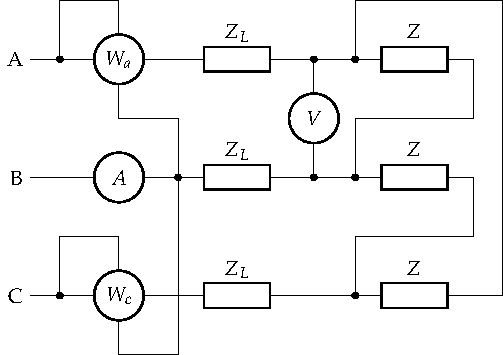
\includegraphics[width = 0.6\textwidth]{../figs/BT3_12}
\end{center}

Dato: $\overline{Z}_L = \SI[parse-numbers = false]{1 + j}{\ohm}$.

\textbf{Sol.: $ Z = \SI[parse-numbers=false]{80\sqrt{3}}{\ohm}$;
  $ I_{a} = {5\phase{91.24^\circ}}\unit{\ampere}$;
  $ I_{b} = {5\phase{-28.75^\circ}}\unit{\ampere}$;
  $ I_{c} = {5\phase{-148.75^\circ}}\unit{\ampere}$;
  $ W_a = W_c = \SI{1761.04}{\watt}$}

\item En el circuito de la figura se debe determinar:

\begin{center}
  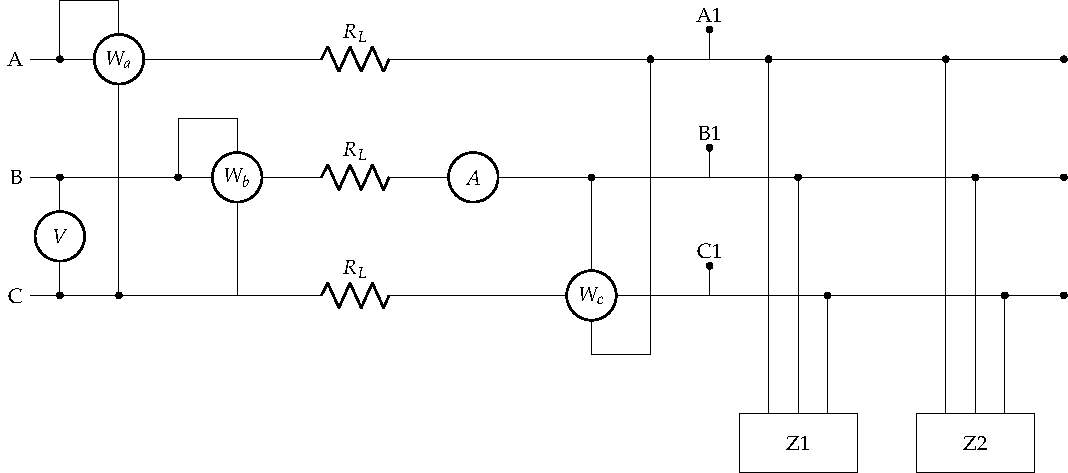
\includegraphics[width=0.9\textwidth]{../figs/BT3_11.pdf}
\end{center}

\begin{enumerate}
\item Lectura del vatímetro $W_c$.
\item Lectura del amperímetro.
\item Factor de potencia total de las cargas (en retraso o adelanto).
\item Lectura de los vatímetros $W_a$ y $W_b$.
\item Lectura del voltímetro.
\item Valor de los condensadores conectados en $A_1B_1C_1$ para que el
  f.d.p. en ese punto sea la unidad.
\item Lecturas de los cinco aparatos de medida tras el apartado
  anterior.
\end{enumerate}

Datos:
\begin{itemize}
\item Secuencia de fases directa, $f = \SI{50}{\hertz}$, ($A_1B_1C_1$)
  $U_1 = \SI{420}{\volt}$.
\item $Z_1$: motor de 10 CV, con $\eta = 0.83$, y f.d.p. de 0'9.
\item $Z_2$: conjunto de iluminación fluorescente, con
  $P = \SI{2400}{\watt}$, y f.d.p. de 0'85.
\item $R_L = \SI{1}{\ohm}$.
\end{itemize}

\textbf{Sol.: $ W_c = \qty{-3338.3}{\watt}$;
  $ A = \SI{17.41}{\ampere}$; $ fdp = 0.89$;
  $ W_A = \SI{7757.6}{\watt}$; $ W_B = \SI{4419.27}{\watt}$;
  $ U' = \SI{447.02}{\volt}$; $ C = \SI{34.78}{\micro\farad}$}

\item Una línea ideal trifásica de 4 hilos alimenta a dos cargas a una
  tensión de $\SI{400}{\volt}$ en secuencia de fases inversa (SFI) y
  frecuencia $\SI{50}{\hertz}$.

  Las cargas tienen las siguientes características:

  \begin{itemize}
  \item Un motor trifásico de $\SI{70}{\kilo\watt}$ y f.d.p. de 0.8.
  \item Un conjunto equilibrado de 90 lámparas fluorescentes. Las
    características de cada lámpara son: potencia de $\SI{12}{\watt}$,
    f.d.p. de 0.7 en retraso, tensión $\SI{230}{\volt}$.
  \end{itemize}

  Con esta información se pide:

  \begin{enumerate}
  \item Conectar adecuadamente los siguientes aparatos de medida antes
    de las cargas.
    \begin{itemize}
    \item Un voltímetro que mida la tensión de línea (etiquetado como
      $V_L$) y otro voltímetro que mida la tensión de fase (etiquetado
      como $V_F$).
    \item Un vatímetro que permita calcular la potencia reactiva total
      del sistema (etiquetado como $W_r$).
    \item Dos vatímetros que, de forma conjunta, permitan calcular la
      potencia activa total del sistema (etiquetados como $W_X$ y
      $W_Y$).
    \end{itemize}
  \item Calcular el valor eficaz de la corriente de línea total.
  \item Calcular la lectura de cada uno de los aparatos de medida del
    primer apartado.
  \item Calcular los condensadores necesarios para mejorar el factor
    de potencia hasta 0,9, indicando cómo se deben conectar.
  \item vez conectados los condensadores del anterior apartado,
    determinar la corriente de línea y la lectura de todos los
    aparatos de medida del apartado 2.
  \end{enumerate}

  \textbf{Sol.: $I = \qty{128.5}{\ampere}$; $V_L = \qty{400}{\volt}$;
    $V_F = \qty{230.9}{\volt}$; $W_r = \qty{30947}{\watt}$;
    $W_X = \qty{20666.5}{\watt}$; $W_Y = \qty{51013.5}{\watt}$;
    $C=\SI{127.2}{\micro\farad}$, $I' = \qty{114}{\ampere}$;
    $W'_X = \SI{25602.2}{W}$; $W'_Y = \SI{45477.8}{W}$;
    $W'_R = \SI{19875.6}{W}$}

\item

  En el sistema de la figura de secuencia de fases directa y
  frecuencia $f=\qty{60}{\hertz}$, se dispone de un receptor
  equilibrado con una potencia total $P_T=\qty{51984}{\watt}$ factor
  de potencia de $0.6$ en retraso. Sabiendo que el amperímetro marca
  $\qty[parse-numbers=false]{76\sqrt{3}}{\ampere}$, determinar:
  \begin{enumerate}
  \item Medida de los vatímetros 1 y 2.
  \item Valor de la impedancia $\overline{Z}$ en forma
    módulo-argumento.
  \item Valor de la capacidad mínima para mejorar el factor de
    potencia a $0.95$ en retraso.
  \item Valor de la impedancia equivalente en estrella.
  \end{enumerate}
  \begin{center}
    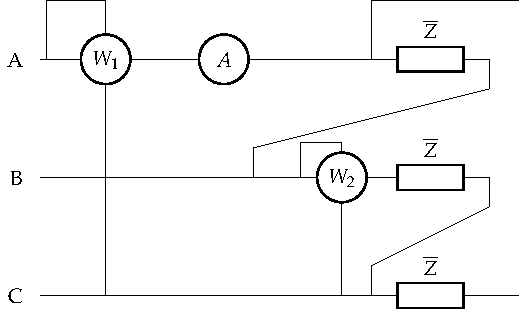
\includegraphics[scale=0.8]{../figs/dosvat_triangulo.pdf}
  \end{center}
  \textbf{Sol.:$W_1 = \qty{46001}{\watt}$; $W_2=\qty{17328}{\watt}$;
    $\overline{Z} = {5\phase{\ang{53.13}}}\unit{\ohm}$.}

\end{enumerate}

%%% Local Variables:
%%% mode: latex
%%% TeX-master: "enunciados_ejercicios_TC"
%%% ispell-local-dictionary: "castellano"
%%% End:


% \chapter{Introducción al régimen transitorio}

% \section*{Ejercicios}
	
\begin{enumerate}
\item El interruptor de la Figura~\ref{fig.ej1_BT4} lleva cerrado un
  tiempo que se puede considerar infinito. En el instante $t=0$, se
  abre, permaneciendo en esta posición definitivamente. Calcular la
  expresión de la intensidad $i(t)$ desde $t=0$ en adelante.
  \begin{figure}[H]
    \centering 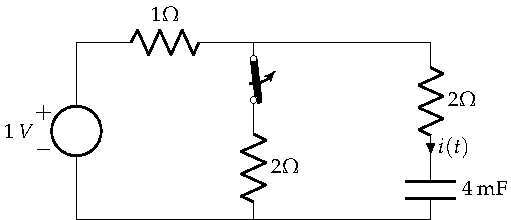
\includegraphics{../figs/ej1_BT4.pdf}
    \caption{Ejercicio 1}
    \label{fig.ej1_BT4}
  \end{figure}
  \emph{Sol.: $i(t)=\dfrac{1}{9}\; \mathrm{e}^{-\frac{t}{0.012}} A$}
\item El circuito de la Figura~\ref{fig.ej2_BT4} se encuentra en
  régimen permanente. En el instante $t=0$ se abre el
  interruptor. Calcular $u_1$ y $u_2$ para $t>0$.
  \begin{figure}[H]
    \centering 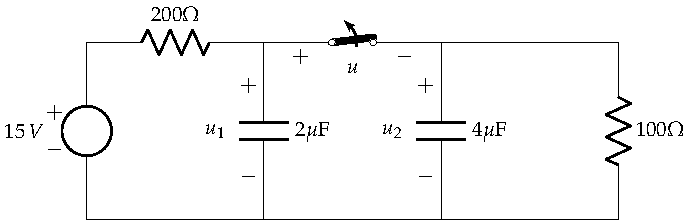
\includegraphics{../figs/ej2_BT4.pdf}
    \caption{Ejercicio 2}
    \label{fig.ej2_BT4}
  \end{figure}
  \emph{Sol.:
    $u_1(t)=15-10\,\mathrm{e}^{-2500\,t}\,V;\;
    u_2(t)=5\,\mathrm{e}^{-2500\,t}\,V$}
\item El interruptor del circuito de la Figura~\ref{fig.ej3_BT4} lleva
  cerrado un timepo que se considera infinito. En el instante $t=0$,
  se abre y permanece en dicha posición definitivamente. Hállese la
  expresión de $u(t)$ e $i(t)$ para $t>0$.
  \begin{figure}[H]
    \centering
    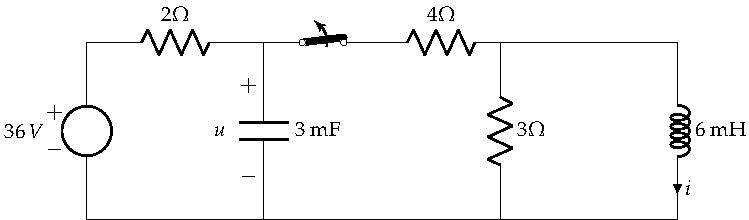
\includegraphics[width=0.65\linewidth]{../figs/ej3_BT4.pdf}
    \caption{Ejercicio 3}
    \label{fig.ej3_BT4}
  \end{figure}
  \emph{Sol.:
    $u(t)=36-12\,\mathrm{e}^{-166.67\,t}\,V;\;
    i(t)=6\,\mathrm{e}^{-500\,t}\,A$}
\item El circuito de la Figura~\ref{fig.ej4_BT4} lleva en esa posición
  un tiempo que se puede considerar infinito. En el instante $t=0$,
  ambos interruptores cambian su posición. Calcular la expresión de
  $u(t)$ para $t>0$.
  \begin{figure}[H]
    \centering
    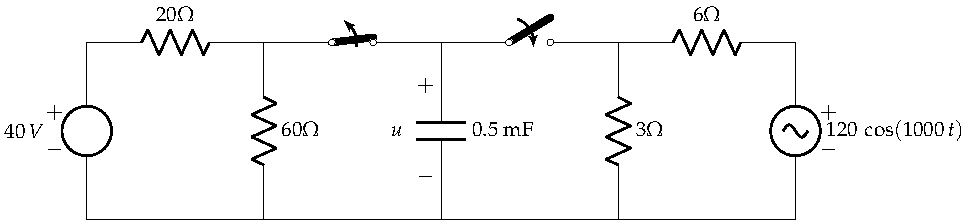
\includegraphics[width=.9\linewidth]{../figs/ej4_BT4.pdf}
    \caption{Ejercicio 4}
    \label{fig.ej4_BT4}
  \end{figure}
  \emph{Sol.:
    $u(t)=10\,\mathrm{e}^{-1000\,t}+20\sqrt{2}\,\cos\left(1000\,t-\frac{\pi}{4}\right)\,V$}
\item En el circuito de la Figura~\ref{fig.ej5_BT4}, se abre el
  interruptor después de un tiempo suficientemente grande para
  considerar que el circuito funcionaba en régimen
  permanente. Expresar las formas de onda de $i_1$, $i_2$ y $u_L$ para
  $t>0$, sabiendo que la fuente de tensión alterna es
  $e(t)=220\sqrt{2}\cos(100\pi\,t)$ V.
  \begin{figure}[H]
    \centering
    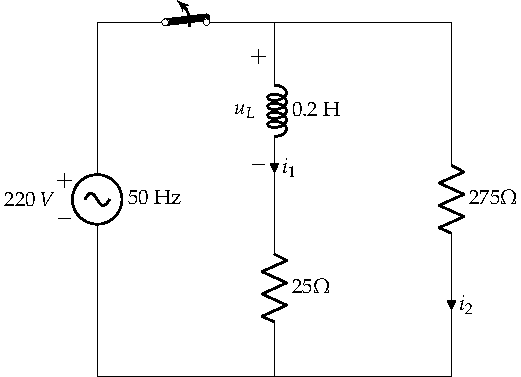
\includegraphics[width=0.45\linewidth]{../figs/ej5_BT4.pdf}
    \caption{Ejercicio 5}
    \label{fig.ej5_BT4}
  \end{figure}
  \emph{Sol.:
    $i_1(t)=1.7\,\mathrm{e}^{-1500\,t}\,A;\;i_2(t)=-1.7\,\mathrm{e}^{-1500\,t}\,A;\;
    u_L(t)=-510\,\mathrm{e}^{-1500\,t}\,V$}
\item En el circuito de la Figura~\ref{fig.ej6_BT4}, en $t = 0$ se
  cierra el interruptor. Obtener la expresión analítica de la
  intensidad $i(t)$, para $t > 0$.
  \begin{figure}[H]
    \centering 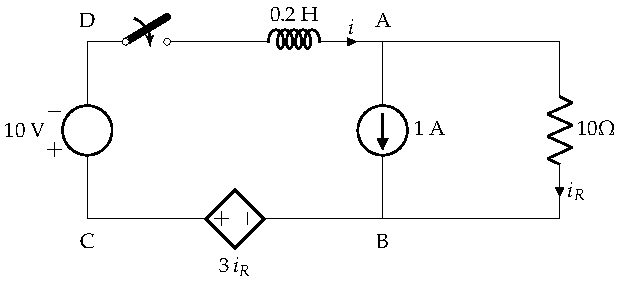
\includegraphics{../figs/ej6_BT4.pdf}
    \caption{Ejercicio 6}
    \label{fig.ej6_BT4}
  \end{figure}
  \emph{Sol.: $i(t)=\dfrac{3}{7}\,\mathrm{e}^{-35\,t}-\dfrac{3}{7}$}
\item En el circuito de la Figura~\ref{fig.ej7_BT4}, el interruptor
  permanece conectado en la posición mostrada el tiempo suficiente
  para que se encuentre en estado estacionario. En el instante $t=0$,
  cambia de posición. Obtener la expresión analítica de la tensión
  entre los bornes de la bobina.
  \begin{figure}[H]
    \centering 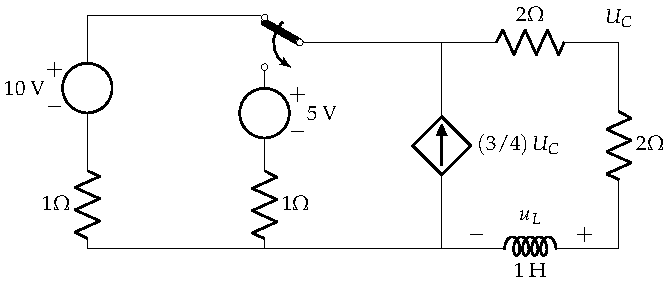
\includegraphics{../figs/ej7_BT4.pdf}
    \caption{Ejercicio 7}
    \label{fig.ej7_BT4}
  \end{figure}
  \emph{Sol.: $u(t)=-20\,\mathrm{e}^{-14\,t}\,V$}
\item En el circuito de la Figura~\ref{fig.FM_4_9}, calcular la tensión $u_C(t)$ para $t > 0$.\\
  Datos:
  $\epsilon_g = 4V;\; R_1 = {2}{\Omega};\; R_2 = {2}{\Omega};\; L =
  {1}{H};\; C = {0.25}{F} $
  \begin{figure}[H]
    \centering 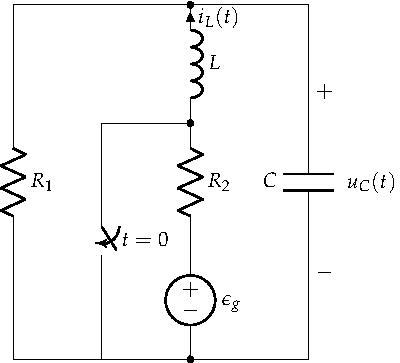
\includegraphics{../figs/FM_4_9.pdf}
    \caption{Ejercicio 8}
    \label{fig.FM_4_9}
  \end{figure}

  \emph{Sol.:
    $u_C(t)=
    \mathrm{e}^{-t}\left[2\,\cos(\sqrt{3}\,t)+\dfrac{2}{\sqrt{3}}\,\sin(\sqrt{3}\,t)\right]=\dfrac{4\sqrt{3}}{3}\,\mathrm{e}^{-t}\,\sin\left(\sqrt{3}\,t+\dfrac{\pi}{6}\right)$
    V}
  % \item El circuito de la Figura~\ref{fig.ej11_BT4} ha alcanzado el
  %   régimen permanente con el
  %   interruptor cerrado. El interruptor se abre en $t = 0$. Calcular las expresiones de la tensión en bornes del condensador y de la corriente por la bobina para $t > 0$.\\
  %   Datos:
  %
  %
  %
  %
  %
  %
  %
  %
  %
  %
  %
  %
  %
  %
  %
  %
  %
  %
  %
  %
  %
  %
  %
  %
  %
  %
  %
  %
  %
  %
  %
  %
  %
  %
  %
  %
  %
  %
  %
  %
  %
  %
  %
  %
  %
  %
  %
  %
  %
  %
  %
  %
  %
  %
  %
  %
  %
  %
  %
  %
  %
  %
  %
  %
  %
  %
  %
  %
  %
  %
  %
  %
  %
  %
  %
  %
  %
  %
  %
  %
  %
  %
  %
  %
  %
  %
  %
  %
  %
  %
  %
  %
  %
  %
  %
  %
  %
  %
  %
  %
  %
  %
  %
  %
  %
  %
  %
  %
  %
  %
  %
  %
  %
  %
  %
  %
  %
  %
  %
  %
  %
  %
  %
  %
  %
  %
  %
  %
  %
  %
  %
  %
  %
  %
  %
  %
  %
  %
  %
  %
  %
  %
  %
  %
  %
  %
  %
  %
  %
  %
  %
  %
  %
  %
  %
  %
  %
  %
  %
  %
  %
  %
  %
  %
  %
  %
  %
  %
  %
  %
  %
  %
  %
  %
  %
  %
  %
  %
  %
  %
  %
  %
  %
  %
  %
  %
  %
  %
  %
  %
  %
  %
  %
  %
  %
  %
  %
  %
  %
  %
  %
  %
  %
  %
  %
  %
  %
  %
  %
  %
  %
  %
  %
  %
  %
  %
  %
  %
  %
  %
  %
  %
  %
  %
  %
  %
  %
  %
  %
  %
  %
  %
  %
  %
  %
  %
  %
  %
  %
  %
  %
  %
  %
  %
  %
  %
  %
  %
  %
  %
  %
  %
  %
  %
  %
  %
  %
  %
  %
  %
  %
  %
  %
  %
  %
  %
  %
  %
  %
  %
  %
  %
  %
  %
  %
  %
  %
  %
  %
  %
  %
  %
  %
  %
  %
  %
  %
  %
  %
  %
  %
  %
  %
  %
  %
  %
  %
  %
  %
  %
  %
  %
  %
  %
  %
  %
  %
  %
  %
  %
  %
  %
  %
  %
  %
  %
  %
  %
  %
  %
  %
  %
  %
  %
  %
  %
  %
  %
  %
  %
  %
  %
  %
  %
  %
  %
  %
  %
  %
  %
  %
  %
  %
  %
  %
  %
  %
  %
  %
  %
  %
  %
  %
  %
  %
  %
  %
  %
  %
  %
  %
  %
  %
  %
  %
  %
  %
  %
  %
  %
  %
  %
  %
  %
  %
  %
  %
  %
  %
  %
  %
  %
  %
  %
  %
  %
  %
  %
  %
  %
  %
  %
  %
  %
  %
  %
  %
  %
  %
  %
  %
  %
  %
  %
  %
  %
  %
  %
  %
  %
  %
  %
  %
  %
  %
  %
  %
  %
  %
  %
  %
  %
  %
  %
  %
  %
  %
  %
  %
  %
  %
  %
  %
  %
  %
  %
  %
  %
  %
  %
  %
  %
  %
  %
  %
  %
  %
  %
  %
  %
  %
  %
  %
  %
  %
  %
  %
  %
  %
  %
  %
  %
  %
  %
  %
  %
  %
  %
  %
  %
  %
  %
  %
  %
  %
  %
  %
  %
  %
  %
  %
  %
  %
  %
  %
  %
  %
  %
  %
  %
  %
  %
  %
  %
  %
  %
  %
  %
  %
  %
  %
  %
  %
  %
  %
  %
  %
  %
  %
  %
  %
  %
  %
  %
  %
  %
  %
  %
  %
  %
  %
  %
  %
  %
  %
  %
  %
  %
  %
  %
  %
  %
  %
  %
  %
  %
  %
  %
  %
  %
  %
  %
  %
  %
  %
  %
  %
  %
  %
  %
  %
  %
  %
  %
  %
  %
  %
  %
  %
  %
  %
  %
  %
  %
  %
  %
  %
  %
  %
  %
  %
  %
  %
  %
  %
  %
  %
  %
  %
  %
  %
  %
  %
  %
  %
  %
  %
  %
  %
  %
  %
  %
  %
  %
  %
  %
  %
  %
  %
  %
  %
  %
  %
  %
  %
  %
  %
  %
  %
  %
  %
  %
  %
  %
  %
  %
  %
  %
  %
  %
  %
  %
  %
  %
  %
  %
  %
  %
  %
  %
  %
  %
  %
  %
  %
  %
  %
  %
  %
  %
  %
  %
  %
  %
  %
  %
  %
  %
  %
  %
  %
  %
  %
  %
  %
  %
  %
  %
  %
  %
  %
  %
  %
  %
  %
  %
  %
  %
  %
  %
  %
  %
  %
  %
  %
  %
  %
  %
  %
  %
  %
  %
  %
  %
  %
  %
  %
  %
  %
  %
  %
  %
  %
  %
  %
  %
  %
  %
  %
  %
  %
  %
  %
  %
  %
  %
  %
  %
  %
  %
  %
  %
  %
  %
  %
  %
  %
  %
  %
  %
  %
  %
  %
  %
  %
  %
  %
  %
  %
  %
  %
  %
  %
  %
  %
  %
  %
  %
  %
  %
  %
  %
  %
  %
  %
  %
  %
  %
  %
  %
  %
  %
  %
  %
  %
  %
  %
  %
  %
  %
  %
  %
  %
  %
  %
  %
  %
  %
  %
  %
  %
  %
  %
  %
  %
  %
  %
  %
  %
  %
  %
  %
  %
  %
  %
  %
  %
  %
  %
  %
  %
  %
  %
  %
  %
  %
  %
  %
  %
  %
  %
  %
  %
  %
  %
  %
  %
  %
  %
  %
  %
  %
  %
  %
  %
  %
  %
  %
  %
  %
  %
  %
  %
  %
  %
  %
  %
  %
  %
  %
  %
  %
  %
  %
  %
  %
  %
  %
  %
  %
  %
  %
  %
  %
  %
  %
  %
  %
  %
  %
  %
  %
  %
  %
  %
  %
  %
  %
  %
  %
  %
  %
  %
  %
  %
  %
  %
  %
  %
  %
  %
  %
  %
  %
  %
  %
  %
  %
  %
  %
  %
  %
  %
  %
  %
  %
  %
  %
  %
  %
  %
  %
  %
  %
  %
  %
  %
  %
  %
  %
  %
  %
  %
  %
  %
  %
  %
  %
  %
  %
  %
  %
  %
  %
  %
  %
  %
  %
  %
  %
  %
  %
  %
  %
  %
  %
  %
  %
  %
  %
  %
  %
  %
  %
  %
  %
  %
  %
  %
  %
  %
  %
  %
  %
  %
  %
  %
  %
  %
  %
  %
  %
  %
  %
  %
  %
  %
  %
  %
  %
  %
  %
  %
  %
  %
  %
  %
  %
  %
  %
  %
  %
  %
  %
  %
  %
  %
  %
  %
  %
  %
  %
  %
  %
  %
  %
  %
  %
  %
  %
  %
  %
  %
  %
  %
  %
  %
  %
  %
  %
  %
  %
  %
  %
  %
  %
  %
  %
  %
  %
  %
  %
  %
  %
  %
  %
  %
  %
  %
  %
  %
  %
  %
  %
  %
  %
  %
  %
  %
  %
  %
  %
  %
  %
  %
  %
  %
  %
  %
  %
  %
  %
  %
  %
  %
  %
  %
  %
  %
  %
  %
  %
  %
  %
  %
  %
  %
  %
  %
  %
  %
  %
  %
  %
  %
  %
  %
  %
  %
  %
  %
  %
  %
  %
  %
  %
  %
  %
  %
  %
  %
  %
  %
  %
  %
  %
  %
  %
  %
  %
  %
  %
  %
  %
  %
  %
  %
  %
  %
  %
  %
  %
  %
  %
  %
  %
  %
  %
  %
  %
  %
  %
  %
  %
  %
  %
  %
  %
  %
  %
  %
  %
  %
  %
  %
  %
  %
  %
  %
  %
  %
  %
  %
  %
  %
  %
  %
  %
  %
  %
  %
  %
  %
  %
  %
  %
  %
  %
  %
  %
  %
  %
  %
  %
  %
  %
  %
  %
  %
  %
  %
  %
  %
  %
  %
  %
  %
  %
  %
  %
  %
  %
  %
  %
  %
  %
  %
  %
  %
  %
  %
  %
  %
  %
  %
  %
  %
  %
  %
  %
  %
  %
  %
  %
  %
  %
  %
  %
  %
  %
  %
  %
  %
  %
  %
  %
  %
  %
  %
  %
  %
  %
  %
  %
  %
  %
  %
  %
  %
  %
  %
  %
  %
  %
  %
  %
  %
  %
  %
  %
  %
  %
  %
  %
  %
  %
  %
  %
  %
  %
  %
  %
  %
  %
  %
  %
  %
  %
  %
  %
  %
  %
  %
  %
  %
  %
  %
  %
  %
  %
  %
  %
  %
  %
  %
  %
  %
  %
  %
  %
  %
  %
  %
  %
  %
  %
  %
  %
  %
  %
  %
  %
  %
  %
  %
  %
  %
  %
  %
  %
  %
  %
  %
  %
  %
  %
  %
  %
  %
  %
  %
  %
  %
  %
  %
  %
  %
  %
  %
  %
  %
  %
  %
  %
  %
  %
  %
  %
  %
  %
  %
  %
  %
  %
  %
  %
  %
  %
  %
  %
  %
  %
  %
  %
  %
  %
  %
  %
  %
  %
  %
  %
  %
  %
  %
  %
  %
  %
  %
  %
  %
  %
  %
  %
  %
  %
  %
  %
  %
  %
  %
  %
  %
  %
  %
  %
  %
  %
  %
  %
  %
  %
  %
  %
  %
  %
  %
  %
  %
  %
  %
  %
  %
  %
  %
  %
  %
  %
  %
  %
  %
  %
  %
  %
  %
  %
  %
  %
  %
  %
  %
  %
  %
  %
  %
  %
  %
  %
  %
  %
  %
  %
  %
  %
  %
  %
  %
  %
  %
  %
  %
  %
  %
  %
  %
  %
  %
  %
  %
  %
  %
  %
  %
  %
  %
  %
  %
  %
  %
  %
  %
  %
  %
  %
  %
  %
  %
  %
  %
  %
  %
  %
  %
  %
  %
  %
  %
  %
  %
  %
  %
  %
  %
  %
  %
  %
  %
  %
  %
  %
  %
  %
  %
  %
  %
  %
  %
  %
  %
  %
  %
  %
  %
  %
  %
  %
  %
  %
  %
  %
  %
  %
  %
  %
  %
  %
  %
  %
  %
  %
  %
  %
  %
  %
  %
  %
  %
  %
  %
  %
  %
  %
  %
  %
  %
  %
  %
  %
  %
  %
  %
  %
  %
  %
  %
  %
  %
  %
  %
  %
  %
  %
  %
  %
  %
  %
  %
  %
  %
  %
  %
  %
  %
  %
  %
  %
  %
  %
  %
  %
  %
  %
  %
  %
  %
  %
  %
  %
  %
  %
  %
  %
  %
  %
  %
  %
  %
  %
  %
  %
  %
  %
  %
  %
  %
  %
  %
  %
  %
  %
  %
  %
  %
  %
  %
  %
  %
  %
  %
  %
  %
  %
  %
  %
  %
  %
  %
  %
  %
  %
  %
  %
  %
  %
  %
  %
  %
  %
  %
  %
  %
  %
  %
  %
  %
  %
  %
  %
  %
  %
  %
  %
  %
  %
  %
  %
  %
  %
  %
  %
  %
  %
  %
  %
  %
  %
  %
  %
  %
  %
  %
  %
  %
  %
  %
  %
  %
  %
  %
  %
  %
  %
  %
  %
  %
  %
  %
  %
  %
  %
  %
  %
  %
  %
  %
  %
  %
  %
  %
  %
  %
  %
  %
  %
  %
  %
  %
  %
  %
  %
  %
  %
  %
  %
  %
  %
  %
  %
  %
  %
  %
  %
  %
  %
  %
  %
  %
  %
  %
  %
  %
  %
  %
  %
  %
  %
  %
  %
  %
  %
  %
  %
  %
  %
  %
  %
  %
  %
  %
  %
  %
  %
  %
  %
  %
  %
  %
  %
  %
  %
  %
  %
  %
  %
  %
  %
  %
  %
  %
  %
  %
  %
  %
  %
  %
  %
  %
  %
  %
  %
  %
  %
  %
  %
  %
  %
  %
  %
  %
  %
  %
  %
  %
  %
  %
  %
  %
  %
  %
  %
  %
  %
  %
  %
  %
  %
  %
  %
  %
  %
  %
  %
  %
  %
  %
  %
  %
  %
  %
  %
  %
  %
  %
  %
  %
  %
  %
  %
  %
  %
  %
  %
  %
  %
  %
  %
  %
  %
  %
  %
  %
  %
  %
  %
  %
  %
  %
  %
  %
  %
  %
  %
  %
  %
  %
  %
  %
  %
  %
  %
  %
  %
  %
  %
  %
  %
  %
  %
  %
  %
  %
  %
  %
  %
  %
  %
  %
  %
  %
  %
  %
  %
  %
  %
  %
  %
  %
  %
  %
  %
  %
  %
  %
  %
  %
  %
  %
  %
  %
  %
  %
  %
  %
  %
  %
  %
  %
  %
  %
  %
  %
  %
  %
  %
  %
  %
  %
  %
  %
  %
  %
  %
  %
  %
  %
  %
  %
  %
  %
  %
  %
  %
  %
  %
  %
  %
  %
  %
  %
  %
  %
  %
  %
  %
  %
  %
  %
  %
  %
  %
  %
  %
  %
  %
  %
  %
  %
  %
  %
  %
  %
  %
  %
  %
  %
  %
  %
  %
  %
  %
  %
  %
  %
  %
  %
  %
  %
  %
  %
  %
  %
  %
  %
  %
  %
  %
  %
  %
  %
  %
  %
  %
  %
  %
  %
  %
  %
  %
  %
  %
  %
  %
  %
  %
  %
  %
  %
  %
  %
  %
  %
  %
  %
  %
  %
  %
  %
  %
  %
  %
  %
  %
  %
  %
  %
  %
  %
  %
  %
  %
  %
  %
  %
  %
  %
  %
  %
  %
  %
  %
  %
  %
  %
  %
  %
  %
  %
  %
  %
  %
  %
  %
  %
  %
  %
  %
  %
  %
  %
  %
  %
  %
  %
  %
  %
  %
  %
  %
  %
  %
  %
  %
  %
  %
  %
  %
  %
  %
  %
  %
  %
  %
  %
  %
  %
  %
  %
  %
  %
  %
  %
  %
  %
  %
  %
  %
  %
  %
  %
  %
  %
  %
  %
  %
  %
  %
  %
  %
  %
  %
  %
  %
  %
  %
  %
  %
  %
  %
  %
  %
  %
  %
  %
  %
  %
  %
  %
  %
  %
  %
  %
  %
  %
  %
  %
  %
  %
  %
  %
  %
  %
  %
  %
  %
  %
  %
  %
  %
  %
  %
  %
  %
  %
  %
  %
  %
  %
  %
  %
  %
  %
  %
  %
  %
  %
  %
  %
  %
  %
  %
  %
  %
  %
  %
  %
  %
  %
  %
  %
  %
  %
  %
  %
  %
  %
  %
  %
  %
  %
  %
  %
  %
  %
  %
  %
  %
  %
  %
  %
  %
  %
  %
  %
  %
  %
  %
  %
  %
  %
  %
  %
  %
  %
  %
  %
  %
  %
  %
  %
  %
  %
  %
  %
  %
  %
  %
  %
  %
  %
  %
  %
  %
  %
  %
  %
  %
  %
  %
  %
  %
  %
  %
  %
  %
  %
  %
  %
  %
  %
  %
  %
  %
  %
  %
  %
  %
  %
  %
  %
  %
  %
  %
  %
  %
  %
  %
  %
  %
  %
  %
  %
  %
  %
  %
  %
  %
  %
  %
  %
  %
  %
  %
  %
  %
  %
  %
  %
  %
  %
  %
  %
  %
  %
  %
  %
  %
  %
  %
  %
  %
  %
  %
  %
  %
  %
  %
  %
  %
  %
  %
  %
  %
  %
  %
  %
  %
  %
  %
  %
  %
  %
  %
  %
  %
  %
  %
  %
  %
  %
  %
  %
  %
  %
  %
  %
  %
  %
  %
  %
  %
  %
  %
  %
  %
  %
  %
  %
  %
  %
  %
  %
  %
  %
  %
  %
  %
  %
  %
  %
  %
  %
  %
  %
  %
  %
  %
  %
  %
  %
  %
  %
  %
  %
  %
  %
  %
  %
  %
  %
  %
  %
  %
  %
  %
  %
  %
  %
  %
  %
  %
  %
  %
  %
  %
  %
  %
  %
  %
  %
  %
  %
  %
  %
  %
  %
  %
  %
  %
  %
  %
  %
  %
  %
  %
  %
  %
  %
  %
  %
  %
  %
  %
  %
  %
  %
  %
  %
  %
  %
  %
  %
  %
  %
  %
  %
  %
  %
  %
  %
  %
  %
  %
  %
  %
  %
  %
  %
  %
  %
  %
  %
  %
  %
  %
  %
  %
  %
  %
  %
  %
  %
  %
  %
  %
  %
  %
  %
  %
  %
  %
  %
  %
  %
  %
  %
  %
  %
  %
  %
  %
  %
  %
  %
  %
  %
  %
  %
  %
  %
  %
  %
  %
  %
  %
  %
  %
  %
  %
  %
  %
  %
  %
  %
  %
  %
  %
  %
  %
  %
  %
  %
  %
  %
  %
  %
  %
  %
  %
  %
  %
  %
  %
  %
  %
  %
  %
  %
  %
  %
  %
  %
  %
  %
  %
  %
  %
  %
  %
  %
  %
  %
  %
  %
  %
  %
  %
  %
  %
  %
  %
  %
  %
  %
  %
  %
  %
  %
  %
  %
  %
  %
  %
  %
  %
  %
  %
  %
  %
  %
  %
  %
  %
  %
  %
  %
  %
  %
  %
  %
  %
  %
  %
  %
  %
  %
  %
  %
  %
  %
  %
  %
  %
  %
  %
  %
  %
  %
  %
  %
  %
  %
  %
  %
  %
  %
  %
  %
  %
  %
  %
  %
  %
  %
  %
  %
  %
  %
  %
  %
  %
  %
  %
  %
  %
  %
  %
  %
  %
  %
  %
  %
  %
  %
  %
  %
  %
  %
  %
  %
  %
  %
  %
  %
  %
  %
  %
  %
  %
  %
  %
  %
  %
  %
  %
  %
  %
  %
  %
  %
  %
  %
  %
  %
  %
  %
  %
  %
  %
  %
  %
  %
  %
  %
  %
  %
  %
  %
  %
  %
  %
  %
  %
  %
  %
  %
  %
  %
  %
  %
  %
  %
  %
  %
  %
  %
  %
  %
  %
  %
  %
  %
  %
  %
  %
  %
  %
  %
  %
  %
  %
  %
  %
  %
  %
  %
  %
  %
  %
  %
  %
  %
  %
  %
  %
  %
  %
  %
  %
  %
  %
  %
  %
  %
  %
  %
  %
  %
  %
  %
  %
  %
  %
  %
  %
  %
  %
  %
  %
  %
  %
  %
  %
  %
  %
  %
  %
  %
  %
  %
  %
  %
  %
  %
  %
  %
  %
  %
  %
  %
  %
  %
  %
  %
  %
  %
  %
  %
  %
  %
  %
  %
  %
  %
  %
  %
  %
  %
  %
  %
  %
  %
  %
  %
  %
  %
  %
  %
  %
  %
  %
  %
  %
  %
  %
  %
  %
  %
  %
  %
  %
  %
  %
  %
  %
  %
  %
  %
  %
  %
  %
  %
  %
  %
  %
  %
  %
  %
  %
  %
  %
  %
  %
  %
  %
  %
  %
  %
  %
  %
  %
  %
  %
  %
  %
  %
  %
  %
  %
  %
  %
  %
  %
  %
  %
  %
  %
  %
  %
  %
  %
  %
  %
  %
  %
  %
  %
  %
  %
  %
  %
  %
  %
  %
  %
  %
  %
  %
  %
  %
  %
  %
  %
  %
  %
  %
  %
  %
  %
  %
  %
  %
  %
  %
  %
  %
  %
  %
  %
  %
  %
  %
  %
  %
  %
  %
  %
  %
  %
  %
  %
  %
  %
  %
  %
  %
  %
  %
  %
  %
  %
  %
  %
  %
  %
  %
  %
  %
  %
  %
  %
  %
  %
  %
  %
  %
  %
  %
  %
  %
  %
  %
  %
  %
  %
  %
  %
  %
  %
  %
  %
  %
  %
  %
  %
  %
  %
  %
  %
  %
  %
  %
  %
  %
  %
  %
  %
  %
  %
  %
  %
  %
  %
  %
  %
  %
  %
  %
  %
  %
  %
  %
  %
  %
  %
  %
  %
  %
  %
  %
  %
  %
  %
  %
  %
  %
  %
  %
  %
  %
  %
  %
  %
  %
  %
  %
  %
  %
  %
  %
  %
  %
  %
  %
  %
  %
  %
  %
  %
  %
  %
  %
  %
  %
  %
  %
  %
  %
  %
  %
  %
  %
  %
  %
  %
  %
  %
  %
  %
  %
  %
  %
  %
  %
  %
  %
  %
  %
  %
  %
  %
  %
  %
  %
  %
  %
  %
  %
  %
  %
  %
  %
  %
  %
  %
  %
  %
  %
  %
  %
  %
  %
  %
  %
  %
  %
  %
  %
  %
  %
  %
  %
  %
  %
  %
  %
  %
  %
  %
  %
  %
  %
  %
  %
  %
  %
  %
  %
  %
  %
  %
  %
  %
  %
  %
  %
  %
  %
  %
  %
  %
  %
  %
  %
  %
  %
  %
  %
  %
  %
  %
  %
  %
  %
  %
  %
  %
  %
  %
  %
  %
  %
  %
  %
  %
  %
  %
  %
  %
  %
  %
  %
  %
  %
  %
  %
  %
  %
  %
  %
  %
  %
  %
  %
  %
  %
  %
  %
  %
  %
  %
  %
  %
  %
  %
  %
  %
  %
  %
  %
  %
  %
  %
  %
  %
  %
  %
  %
  %
  %
  %
  %
  %
  %
  %
  %
  %
  %
  %
  %
  %
  %
  %
  %
  %
  %
  %
  %
  %
  %
  %
  %
  %
  %
  %
  %
  %
  %
  %
  %
  %
  %
  %
  %
  %
  %
  %
  %
  %
  %
  %
  %
  %
  %
  %
  %
  %
  %
  %
  %
  %
  %
  %
  %
  %
  %
  %
  %
  %
  %
  %
  %
  %
  %
  %
  %
  %
  %
  %
  %
  %
  %
  %
  %
  %
  %
  %
  %
  %
  %
  %
  %
  %
  %
  %
  %
  %
  %
  %
  %
  %
  %
  %
  %
  %
  %
  %
  %
  %
  %
  %
  %
  %
  %
  %
  %
  %
  %
  %
  %
  %
  %
  %
  %
  %
  %
  %
  %
  %
  %
  %
  %
  %
  %
  %
  %
  %
  %
  %
  %
  %
  %
  %
  %
  %
  %
  %
  %
  %
  %
  %
  %
  %
  %
  %
  %
  %
  %
  %
  %
  %
  %
  %
  %
  %
  %
  %
  %
  %
  %
  %
  %
  %
  %
  %
  %
  %
  %
  %
  %
  %
  %
  %
  %
  %
  %
  %
  %
  %
  %
  %
  %
  %
  %
  %
  %
  %
  %
  %
  %
  %
  %
  %
  %
  %
  %
  %
  %
  %
  %
  %
  %
  %
  %
  %
  %
  %
  %
  %
  %
  %   $\epsilon_g = {10}{V};\; R_1 = {10}{\Omega};\; R_2 = {5}{\Omega};\;L = {2.5}{H};\; C = {0.2}{F}$
% \begin{figure}[H]
%     \centering
%     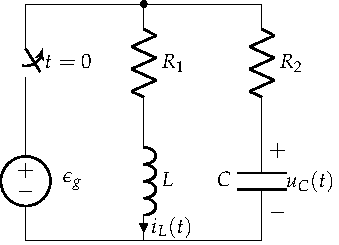
\includegraphics{../figs/FM_4_8.pdf}
%     \caption{Ejercicio 11}
%     \label{fig.ej11_BT4}
% \end{figure}

% \emph{Sol.: $i_L(t)=0.651\,\mathrm{e}^{0.317\,t}+0.349\,\mathrm{e}^{-6.317\,t};\; u_C(t)=10.281\,\mathrm{e}^{0.317\,t}-0.277\,\mathrm{e}^{-6.317\,t}$ A}
\item En el circuito de la Figura~\ref{fig.ej12_BT4} el interruptor ha estado cerrado durante un tiempo elevado y, en $t = 0$, se abre. Determinar la expresión de la corriente $i_L(t)$ para $t>0$, especificando el tipo de transitorio.\\
Datos: $E_g = 500 V;\; R_1 = 375 \Omega;\; R_2 = 125\Omega;\; L_1 = 40 mH;\; L_2 = 40 mH;\; C = 1 \mu F$
\begin{figure}[H]
    \centering
    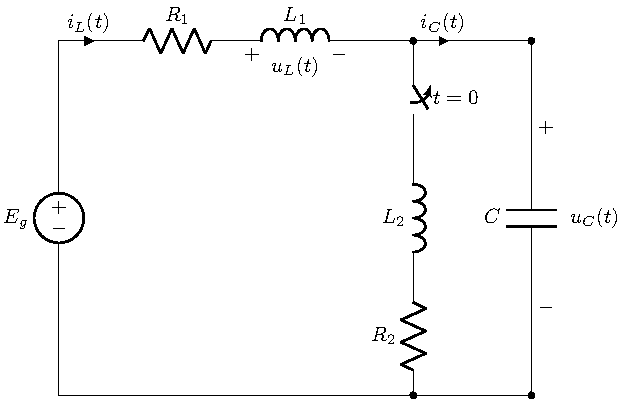
\includegraphics{../figs/ej12_BT4.pdf}
    \caption{Ejercicio 9}
    \label{fig.ej12_BT4}
\end{figure}

	   \emph{Sol.: $i_L(t)= \mathrm{e}^{-4687.5\,t}\left[\cos(1739.93\,t)+2.69\,\sin(1739.93\,t)\right]=2.87\,\mathrm{e}^{-t}\,\sin\left(1739.93\,t+1.215\right)$ A}
	    
\item En el circuito de la Figura~\ref{fig.ej11_BT4}, determinar la tensión $u$ en el condensador a partir del instante en que se abre el interruptor, el cual lleva cerrado desde un tiempo infinito.
\begin{figure}[H]
    \centering
    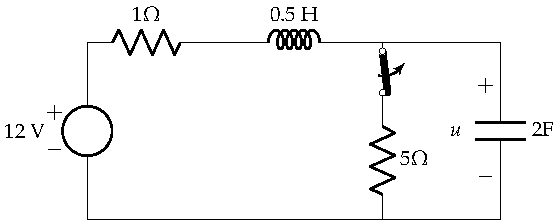
\includegraphics{../figs/ej11_BT4.pdf}
    \caption{Ejercicio 10}
    \label{fig.ej11_BT4}
\end{figure}	 
\emph{Sol.: $u(t)=12-\mathrm{e}^{-t}\left(2+2\,t\right)$ V}

	    
	   % \item El circuito de la Figura~\ref{fig.ej10_BT4} se encuentra en régimen permanente, con el condensador descargado. En un instante dado, que se toma como origen de tiempos, se cierra el interruptor. Determinar $u(t)$ para $t>0$. 
	   % \begin{figure}[H]
	   %     \centering
	   %     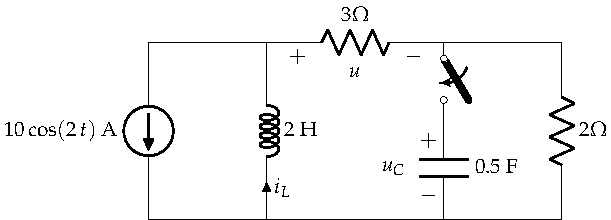
\includegraphics{../figs/ej10_BT4.pdf}
	   %     \caption{Ejercicio 10}
	   %     \label{fig.ej10_BT4}
	   % \end{figure}
	    
	\end{enumerate}
 
%%% Local Variables:
%%% mode: latex
%%% TeX-master: "enunciados_ejercicios_TC"
%%% ispell-local-dictionary: "castellano"
%%% End:



\backmatter


\end{document}

%%% Local Variables:
%%% mode: latex
%%% TeX-master: t
%%% ispell-local-dictionary: "castellano"
%%% End:
